%===============================================================================
%=======     Document Information     ==========================================
%===============================================================================

\title{CS 677: Assignment 7}
\author{Terence Henriod}
\date{\today}
\documentclass[11pts]{article}


%===============================================================================
%=======     Packages Used     =================================================
%===============================================================================

%\usepackage{qtree}
\usepackage{amsmath}
\usepackage{amssymb}
\usepackage[named]{algo}
\usepackage{verbatim}
\usepackage{graphicx}
  \DeclareGraphicsExtensions{.pdf,.png,.jpg}
\usepackage[right=1in,top=1in,left=1in,bottom=1in]{geometry}


%===============================================================================
%=======     Document Settings     =============================================
%===============================================================================

\setlength{\topmargin}{-1cm}
\setlength{\oddsidemargin}{0in}
\setlength{\textwidth}{6.5in}
\setlength{\textheight}{8.3in}


%%Currently default settings for indentation and symbols.
%%Try these by uncommenting this block!!!
%%Redefine the first level symbols
%\renewcommand{\theenumi}{\fnsymbol{enumi}-}
%\renewcommand{\labelenumi}{\theenumi}
%
%%Redefine the second level symbols
%\renewcommand{\theenumii}{\alph{enumii})}
%\renewcommand{\labelenumii}{\theenumii}
%
%%Redefine the third level symbols
%\renewcommand{\theenumiii}{\roman{enumiii}.}
%\renewcommand{\labelenumiii}{\theenumiii}
%
%%Options for redefining levels


%\arabic
%\alph 
%\Alph
%\roman
%\Roman
%\fnsymbol
%This ^^^ is all you need to change!!


%===============================================================================
%=======     User Defined Commands     =========================================
%===============================================================================

\newcommand{\BigO}[1]{\ensuremath{\operatorname{O}\bigl(#1\bigr)}}
\newcommand{\BigTheta}[1]{\ensuremath{\operatorname{\Theta}\bigl(#1\bigr)}}
\newcommand{\BigOmega}[1]{\ensuremath{\operatorname{\Omega}\bigl(#1\bigr)}}


%===============================================================================
%=======     The Document     ==================================================
%===============================================================================
\begin{document}

\maketitle

%~~~~~~~~~~~~~~~~~~~~~~~~~~~~~~~~~~~~~~~~~~~~~~~~~~~~~~~~~~~~~~~~~~~~~~~~~~~~~~~
%~~~~~~~     Abstract     ~~~~~~~~~~~~~~~~~~~~~~~~~~~~~~~~~~~~~~~~~~~~~~~~~~~~~~
%~~~~~~~~~~~~~~~~~~~~~~~~~~~~~~~~~~~~~~~~~~~~~~~~~~~~~~~~~~~~~~~~~~~~~~~~~~~~~~~
\begin{abstract}
In this assignment, various greedy algorithm problems and related ones are
presented.
\end{abstract}
\newpage

% begin the problem set
\begin{enumerate}
%~~~~~~~~~~~~~~~~~~~~~~~~~~~~~~~~~~~~~~~~~~~~~~~~~~~~~~~~~~~~~~~~~~~~~~~~~~~~~~~
%~~~~~~~     Number 1     ~~~~~~~~~~~~~~~~~~~~~~~~~~~~~~~~~~~~~~~~~~~~~~~~~~~~~~
%~~~~~~~~~~~~~~~~~~~~~~~~~~~~~~~~~~~~~~~~~~~~~~~~~~~~~~~~~~~~~~~~~~~~~~~~~~~~~~~
\item Answer the questions below regarding the following graph:
\begin{verbatim}
                          (e)             (f)
                           |               |
                           |               |
                           | 17            | 15
                           |               |
                     3     |     10        |      1
          (A)-------------(c)-------------(g)---------(h)
           |               |               |         /
           |               |               | 11    /
           | 7             | 9             |     /  5
           |               |               |   /
           |        12     |      14       | /
          (b)-------------(d)-------------(i)
\end{verbatim}

\begin{enumerate}
  %-----------------------------------------------------------------------------
  %-------     A     -----------------------------------------------------------
  %-----------------------------------------------------------------------------
  \item In what order are edges added to the Minimum Spanning Tree
  (MST) using Kruskal's Algorithm? List the edges by giving their endpoints. \\

  \textbf{Solution:} Kruskal's algorithm is carried out by first sorting
  the edges by weight, then selecting edges that have the least weight, but
  that still add to the span of the tree that is forming
  without producing a circuit/cycle. \\

  A more canonical way to view Kruskal's algorithm is that one starts
  with a forrest of trees consisting of a solitary vertex each. Then
  edges are added light to heavy only if the edge would connect two
  trees to form a larger tree. This continues until the largest tree(s)
  possible are formed.\\

  The table below has the edges sorted and the decision of whether or not
  to include the edge in the spanning tree: \\
    \begin{center}
    \begin{tabular}{| c | c | c | c |}
      \hline
        $n^{th}$ edge added & Edge   & Weight & Decision \\
      \hline \hline
           1                & (g, h) &    1   & Keep     \\
      \hline
           2                & (A, c) &    3   & Keep     \\
      \hline
           3                & (h, i) &    5   & Keep     \\
      \hline
           4                & (A, b) &    7   & Keep     \\
      \hline
           5                & (c, d) &    9   & Keep     \\
      \hline
           6                & (c, g) &   10   & Keep     \\
      \hline
                            & (g, i) &   11   & Ignore   \\
      \hline
                            & (b, d) &   12   & Ignore   \\
      \hline
                            & (d, i) &   14   & Ignore   \\
      \hline
           7                & (f, g) &   15   & Keep     \\
      \hline
           8                & (e, c) &   17   & Keep     \\
      \hline
    \end{tabular}
    \end{center}

  \newpage
  %-----------------------------------------------------------------------------
  %-------     B     -----------------------------------------------------------
  %-----------------------------------------------------------------------------
  \item In what order are edges added to the MST using Prim's
  Algorithm starting from vertex A? List the edges by giving their
  endpoints. \\

  \textbf{Solution:} Prim's algorithm essentially starts with an arbitrary
  vertex and then grows the spanning tree by adding the lightest edge 
  (and its associated vertex) that
  will grow the most current version of the spanning tree.\\

  The following table displays the edges as they are added to the tree:

    \begin{center}
    \begin{tabular}{| c | c | c |}
      \hline
        $n^{th}$ edge added & Edge   & Weight \\
      \hline \hline
           1                & (A, c) &    3 \\
      \hline
           2                & (A, b) &    7 \\
      \hline
           3                & (c, d) &    9 \\
      \hline
           4                & (c, g) &   10 \\
      \hline
           5                & (g, h) &    1 \\
      \hline
           6                & (h, i) &    5 \\
      \hline
           7                & (g, f) &   15 \\
      \hline
           8                & (c, e) &   17 \\
      \hline
    \end{tabular}
    \end{center}
  \end{enumerate}

\newpage
%~~~~~~~~~~~~~~~~~~~~~~~~~~~~~~~~~~~~~~~~~~~~~~~~~~~~~~~~~~~~~~~~~~~~~~~~~~~~~~~
%~~~~~~~     Number 2     ~~~~~~~~~~~~~~~~~~~~~~~~~~~~~~~~~~~~~~~~~~~~~~~~~~~~~~
%~~~~~~~~~~~~~~~~~~~~~~~~~~~~~~~~~~~~~~~~~~~~~~~~~~~~~~~~~~~~~~~~~~~~~~~~~~~~~~~
\item Exercise 22.2-9 (page 602): Let $G = ( V, E )$ be a connected,
undirected graph. Give an \BigO{ V + E } time algorithm to compute a path in
$G$ that traverses each edge in $E$ exactly once in each direction. Describe
how you can find your way out of a maze if you are given a large
supply of pennies.\\

  \textbf{Solution:} By modifying the traditional Depth First Search (DFS)
  algorithm, we can identify a path that would traverse every edge in a graph
  precisely twice. The Depth First Search algorithm already explores all
  edges in a graph. In order to track the order in which the edges are
  traversed, we simply need to add a list to the algorithm that lists each
  vertex as it is examined in the DFS-Visit procedure. Once the algorithm
  terminates, the list will contain an order in which to travel to each
  vertex, thus crossing each edge twice. \\

  It is known that DFS is a \BigTheta{ |V| + |E| } algorithm, so it
  satisfies the problem requirement. \\

  In the case of the maze, consider every branching or termination of a path
  a vertex, and thus every path as an edge. Upon embarking on a path,
  one could leave a penny at the start of that path, and upon leaving the
  path, drop another penny. After taking a path, if one reaches a dead end,
  then they must return to the last ``vertex" they were at (dropping a penny
  to show that the path was taken, of course), and at the beginning of the
  path, they should place a second penny. One should prefer paths not
  marked by pennies when confronted with a choice, and never take a
  path that has been marked with 2 pennies. By traversing the maze in
  this manner, one will eventually find the end without exploring any
  path more than necessary (not counting making unlucky choices that
  lead to dead ends, of course). \\

\newpage
%~~~~~~~~~~~~~~~~~~~~~~~~~~~~~~~~~~~~~~~~~~~~~~~~~~~~~~~~~~~~~~~~~~~~~~~~~~~~~~~
%~~~~~~~     Number 3     ~~~~~~~~~~~~~~~~~~~~~~~~~~~~~~~~~~~~~~~~~~~~~~~~~~~~~~
%~~~~~~~~~~~~~~~~~~~~~~~~~~~~~~~~~~~~~~~~~~~~~~~~~~~~~~~~~~~~~~~~~~~~~~~~~~~~~~~
\item Exercise 22.5-6 (page 621): Given a directed graph $G = ( V, E )$
explain how to create another graph $G' = ( V, E )$ such that (a) $G'$ has
the same strongly connected components as $G$, (b) $G'$
has the same component graph as $G$, and (c) $E$ is as small as
possible. Describe a fast algorithm to compute $G'$. \\

  \textbf{Solution:} In short, we need a method that will identify the
  strongly connected components (SCCs) of $G$, then once the strongly
  connected components have been identified, then just enough arcs
  should be added to make the would be SCCs of $G'$ actually be
  strongly connected, and then just enough arcs to connect the SCCs to
  one another to produce a component graph similar to that of $G$. Note
  that $G'$ does not actually need to be constructed directly from the
  elements of $G$, it just has to have matching components; this means
  that we are actually free to create arcs as needed instead of selecting
  from the arc set of $G$, but a similar vertex set is required in order
  to have the same components. \\

  Intuitively, start with the algorithm from the text that identifies the
  SCCs of a graph by performing two depth first searches, one
  on $G$ and one on $G^{T}$, STRONGLY-CONNECTED-COMPONENTS. This
  takes \BigO{|V| + |E|} time. Now we have various subsets of vertices
  that will constitute the SCCs that we need to match. \\

  Now, to ensure that the SCCs are actually strongly connected, we need to add
  arcs that accomplish this. This is most easily done by making one simple
  cycle that runs through all of the vertices of an SCC. We accomplish this
  by constructing what is basically a ``linked list" of the vertices, which
  produces |SCC| - 1 arcs, and add an additional arc that connects the last
  vertex back to the first, giving a total of |SCC| arcs. We do this for all
  SCCs, meaning we add a total of $V$ arcs, for a running time of
  \BigO{|V|}. \\

  Finally, for each pair of SCCs, we create an arc to connect the pair
  in a way that matches the component graph of $G$. This operation takes
  \BigO{|E|} time in terms of the size of the arc set of the component
  graph of $G$. (If we feel it necessary to create the component graph of
  $G$ for reference while constructing $G'$, this construction is known
  to be a \BigO{|V| + |E|} operation) \\

  The algorithm described will have a total running time of
  \BigO{|V| + |E|} + \BigO{|V|} + \BigO{|E|} = \BigO{|V| + |E|}. \\

\newpage
%~~~~~~~~~~~~~~~~~~~~~~~~~~~~~~~~~~~~~~~~~~~~~~~~~~~~~~~~~~~~~~~~~~~~~~~~~~~~~~~
%~~~~~~~     Number 4     ~~~~~~~~~~~~~~~~~~~~~~~~~~~~~~~~~~~~~~~~~~~~~~~~~~~~~~
%~~~~~~~~~~~~~~~~~~~~~~~~~~~~~~~~~~~~~~~~~~~~~~~~~~~~~~~~~~~~~~~~~~~~~~~~~~~~~~~
\item Exercise 24.3-2 (page 663): Give a simple example of a directed
graph with negative-weight edges for which
Dijkstra’s algorithm produces incorrect answers. Why doesn’t the proof of
Theorem 24.6 go through when negative-weight edges are allowed? \\

  \textbf{Solution:} Djikstra's algorithm can fail when negative edge
  weights are allowed due to the fact that vertices are not ``re-visited"
  and the order in which vertices are considered can affect when a
  negative edge weight is considered. For example, in the graph below,
  because $w(S, e) < w(S, a)$, $e$ is addressed before $a$ when relaxing
  edges. This happens again, where $d$ is considered before $b$ in the
  relaxation step for the same reason as before. This makes it so $e$
  cannot be reached again for relaxation since both $s$ and $d$ have been
  examined in the steps that relax arcs emanating from those respective
  vertices. This causes the algorithm to fail since the negative edge is
  considered in the relaxation process too late in the algorithm's execution. \\

\begin{verbatim}
                   1
          (s)>----------->(e)
           V               ^
           | 8             | 1
           |               |
           V       1       ^ 
          (a)-------------(d)
           V               ^
           |               |
           | 8             | 1
           |               |
           V     -8888     ^
          (b)>----------->(c)
\end{verbatim}

    \begin{left}
    \begin{tabular}{| c | c |}
      \hline
        Edge   & Weight \\
      \hline \hline
        (S, a) &     8 \\
      \hline
        (S, e) &     1 \\
      \hline
        (a, b) &     8 \\
      \hline
        (a, d) &     1 \\
      \hline
        (b, c) & -8888 \\
      \hline
        (c, d) &     1 \\
      \hline
        (d, e) &     1 \\
      \hline
    \end{tabular}
    \end{left} \\

  The proof of Theorem 24.6 ``doesn't go through" because the proof assumes
  that because there are no negative edges in the graph that
  $y.d \le u.d$, implying that $\delta(s, y) \le \delta(s, u)$. However, it
  could be that a negative edge exists in the path from $y$ to $u$,
  thus violating the assumption required for the proof. If
  $y.d > u.d$, then we can't be certain that
  $\delta(s, y) \le \delta(s, u) \le u.d$ when $u$ is added to $s$, and the
  constradiction cannot be found.
%                 Make better?

\newpage
%~~~~~~~~~~~~~~~~~~~~~~~~~~~~~~~~~~~~~~~~~~~~~~~~~~~~~~~~~~~~~~~~~~~~~~~~~~~~~~~
%~~~~~~~     Number 5     ~~~~~~~~~~~~~~~~~~~~~~~~~~~~~~~~~~~~~~~~~~~~~~~~~~~~~~
%~~~~~~~~~~~~~~~~~~~~~~~~~~~~~~~~~~~~~~~~~~~~~~~~~~~~~~~~~~~~~~~~~~~~~~~~~~~~~~~
\item Exercise 25.1-6 (page 692): Suppose we also wish to compute the
vertices on shortest paths in the algorithms of
this section. Show how to compute the predecessor
matrix $\Pi$ from the completed
matrix $L$ of shortest-path weights in \BigO{n^3} time. \\

  \textbf{Solution:} If we know the weight of the shortest paths for all
  pairs (since we are given $L$), we can see if a vertex is a(n) (immediate)
  predecessor to another on a shortest path. Consider a pair of vertices
  $i$ and $j$, where $i$ is the ``source" vertex and $j$ is the destination.
  We can determine if another vertex $k$ is a predecessor to $j$ on that
  shortest path if the (shortest) weight of the path from
  $k$ to $j$ complements the
  path from $i$ to $k$, that is, if the path from $i$ to $k$ and the final edge
  from $k$ to $j$ have the same sum as the shortest path from $i$ to $j$, then
  $k$ must be a valid predecessor to $j$ on the shortest path. \\

  Thus, by considering every pair of start and end vertices, and then
  checking every vertex to see if it is a possible predecessor on the shortest
  path between the pair, we can find the predecessors of every vertex on
  a shortest path. \\

  Note that it is possible that there could be multiple such $k$ vertices,
  since there could be multiple equivalent shortest paths from $i$ to $j$;
  the algorithm to be presented will only store the last such predecessor
  considered. The algortihm will produce a possibility for the predecessor
  matrix. Also note that we don't need to concern ourselves with which
  shortest path the predecessor matrix will correspond to, since the matrix
  $L$ does not contain this information anyway.

  Since for each of $n$ initial/start vertices we are checking $n$ end
  vertices to form a pair, and we then check $n$ intermediate vertices,
  this algorithm is \BigO{n * n * n} = \BigO{n^3}, as was specified. \\

  Also note that the weights matrix or an edge weight function is also
  needed for this algorithm; the problem statement neglected to mention this. \\

  The algortihm is defined as follows:
\begin{algorithm}{FIND-PREDECESSORS}[ L((1...n)(1...n)), W((1...n)(1...n)) ]{
  \qcomment{Input: The shortest paths adjacency matrix and the simple edge
                   weights adjacency matrix.} }
  Create \Pi((1...n)(1...n)) \\
  \qfor{i \qlet 1 \qto n} \\
  \qdo
    \qfor{j \qlet 1 \qto n} \\
    \qdo
      \pi_{i,j} = \qnil \\
    \qrof \\
  \qrof \\

  \qfor{ i \qlet 1 \qto n } \\
  \qdo
    \qfor{ j \qlet 1 \qto n }\\
    \qdo
      \qfor{ k \qlet 1 \qto n }\\
      \qdo \\
        \qif{ $l_{i,j}$ = $l_{ik}$ + $w(k, j)$ } \\
        \qthen
            \pi_{i,j} = k
        \qfi
      \qrof
    \qrof
  \qrof
  
\end{algorithm}

\newpage
%~~~~~~~~~~~~~~~~~~~~~~~~~~~~~~~~~~~~~~~~~~~~~~~~~~~~~~~~~~~~~~~~~~~~~~~~~~~~~~~
%~~~~~~~     Number 6     ~~~~~~~~~~~~~~~~~~~~~~~~~~~~~~~~~~~~~~~~~~~~~~~~~~~~~~
%~~~~~~~~~~~~~~~~~~~~~~~~~~~~~~~~~~~~~~~~~~~~~~~~~~~~~~~~~~~~~~~~~~~~~~~~~~~~~~~
\item Exercise 24.3-6 (page 663): We are given a directed graph
$G = ( V, E )$ on which each edge $( u, v ) \in E$ has an
associated value $r( u, v )$, which is a real number in the range
$0 \le r( u, v ) \le 1$ that
represents the reliability of a communication channel from vertex $u$
to vertex $v$.
We interpret $r( u, v )$ as the probability that the channel
from $u$ to $v$ will not fail,
and we assume that these probabilities are independent. Give an efficient
algorithm to find the most reliable path between two given vertices.\\

  \textbf{Solution:} First, since the probabilities are all independent,
  we know that all probabilities will have the largest product. This problem
  in itself displays an optimal substructure, since the largest product
  will have the largest operands. Further, since we are discussing
  communication channels that must follow one another, we know that the
  probability that a channel will not fail will be its own probability
  multiplied with the largest probability of success up to that point. \\

  Second, this problem very closely resembles a ``shortest paths" problem.
  We can use the same algorithms for finding a shortest path by replacing
  addition with multiplication of edge weights, and selecting the maximum
  result instead of the minimum.

  Finally, it is known that shortest path between a pair algorithms are not
  better than single source or single destination shortest path algorithms,
  we will not concern ourselves with the best path between only a particular
  pair. In fact, since we are not given any indication of which vertices/paths
  to consider, we may as well just compute the best paths between all vertices.

  Thus, the task can be accomplished by modifying one line of the
  Floyd-Warshall algorithm from \\
  $d_{i,j}^{(k)} = min( d_{i,j}^{(k-1)}, d_{i,k}^{(k-1)} + d_{k,j}^{(k-1)} )$
  to \\
  $d_{i,j}^{(k)} = max( d_{i,j}^{(k-1)}, d_{i,k}^{(k-1)} * d_{k,j}^{(k-1)} )$,
  giving a \BigTheta{V^{3}} time algorithm.

\end{enumerate}
%\LAST PAGE
\end{document}



















































% begin the problem set
\begin{enumerate}
%~~~~~~~~~~~~~~~~~~~~~~~~~~~~~~~~~~~~~~~~~~~~~~~~~~~~~~~~~~~~~~~~~~~~~~~~~~~~~~~
%~~~~~~~     Number 1     ~~~~~~~~~~~~~~~~~~~~~~~~~~~~~~~~~~~~~~~~~~~~~~~~~~~~~~
%~~~~~~~~~~~~~~~~~~~~~~~~~~~~~~~~~~~~~~~~~~~~~~~~~~~~~~~~~~~~~~~~~~~~~~~~~~~~~~~
\item A search engine company needs to do a significant amount of
computation every time it recompiles its index. For this task, the
company has a single large supercomputer, and an unlimited supply
of high-end PCs. \\
 
They have broken the overall computation into $n$ distinct jobs,
labeled $J_1, J_2, \dots, J_n$, which can be performed completely
independently of one another. Each job consists of two stages: first
it needs to be preprocessed on the supercomputer, and then it needs to 
be finished on one of the PCs. Let’s say that job $J_i$ needs $p_i$
seconds of time on the supercomputer, followed by $f_i$ seconds of
time on a PC. \\

Since there are at least $n$ PCs available on the
premises, the finishing of the jobs can be performed fully in
parallel – all the jobs can be processed at the same time. 
However, the supercomputer can only work on a single job at a
time, so the system managers need to work out an order in which to
feed the jobs to the supercomputer. As soon as the first job in
order is done on the supercomputer, it can be handed off to a PC for 
finishing; at that point in time a second job can be fed to the
supercomputer; when the second job is done on the supercomputer, it
can proceed to a PC regardless of whether or not the first job is done
(since the PCs work in parallel); and so on. \\

Let’s say that a \emph{schedule}
is an ordering of the jobs for the supercomputer, and the \emph{completion
time} of the schedule is the earliest time at which all jobs will have
finished processing on the PCs. This is an important quantity to minimize,
since it determines how rapidly \textbf{\textit{\underline{El Goog}}} can
generate a new index. \\

Give a polynomial-time algorithm that finds a schedule with as small a 
completion time as possible. \\

\textit{Note}: to prove that your greedy strategy yields the optimal
solution, you have to prove that the problem has the greedy-choice property. \\

  \textbf{Solution:} Intuitively, no matter what order we schedule for the
  jobs to run, the last job must wait for $\sum_{i=1}^{n}{p_i}$ before
  finalizing, then it must finalize. It would be a good idea to minimize
  the completion time of this last job, we should put the shortest finishing
  time job last (or another way, the job with the longest finishing time
  first), in order to minimize $\sum_{i=1}^{n}{p_i} + f_n$. This is somewhat
  counter intuitive because we disregard the possibility of maximizing the
  parallelism, but as will be shown, this particular greedy strategy leads
  to the optimal solution. \\

  A greedy algorithm that would solve the problem in
  polynomial time would choose jobs with the longest finishing time first,
  disregarding the pre-processing times. In order to accomplish this, we
  can simply sort the jobs using an $n\lg{n}$ sorting algorithm, and feed
  the jobs into the system with the sorted order. \\

  \textit{The Algorithm} \\
\begin{algorithm}{INDEX-REBUILD}[ J( 0 \dots n - 1 ) ]{
  \qcomment{Input: A list/array of jobs for index recompilation} }

  \qproc[J, 0, n - 1]{RANDOMIZED-QUICKSORT} \\
  \qcom{This is the same as regular quicksort except instead of comparing
        elements directly, it only compares $J[i].f$s} \\
  \qfor{ $i \qlet 0$ \qto $n-1$ } \\
  \do \\
    feed a job to the super-computer \\
    wait for the job to finish pre-processing \\
    send the job to a PC after pre-processing to finish
  \qrof \\
  \qstop \qcom{ After jobs complete at the PCs, the index is recompiled. }
  
\end{algorithm}


  \textit{Greedy Choice} \\
  This algorithm is greedy because it makes the local optimum choice of
  selecting the longest finishing time job first, regardless of
  preprocessing times. \\
  
  \textit{Greedy Choice Property} \\
  To first prove the greedy choice of shortest pre-processing time first,
  consider the completion times $c_i$ for each job, where
  $c_j = \sum_{i=1}^{n}{p_i} + f_j$ since,
  clearly, the pre-processing completion times of each job depend on the
  jobs that pre-process before them.

  Suppose that in the optimal solution the jobs run in some
  order where the $k^{th}$ job has the longest completion time $c_k$, and
  is not first job in the sequence. Also consider the shortest job,
  identified as the $j^{th}$ job. To keep things simple, consider a set
  comprised of just a pair of jobs (i.e. $n=2$). In the ``optimal" solution,
  if the completion time of the job with the longer finishing time is the job
  with the higher completion time, then the greedy solution improves on it by
  reducing the completion time of the job with te longer finishing time and
  still is not any worse because
  $\sum_{i=1}^{n}{p_i} + f_j < \sum_{i=1}^{n}{p_i} + f_k$, so even if the
  change results in the job with the shorter finishing time becoming the
  job with the higher completion time, it is still better than the
  optimal solution. Clearly, the greedy choice is a valid strategy.

  In an inductive manner, this logic can be expanded to a set of
  any size by ordering the jobs
  by arranging
  them pair-wise in order to achieve the best pair-wise absolute
  completion times, and repeating until no improvements can be made,
  because finding a way to reduce the completion time of onw job does
  not result in the increase of the completion time of another job in a
  way that will negate the benefits of the change. \\

  The greedy choice of choosing the job with the longest finishing
  time first has improved on what we had originally assumed to be the
  optimal solution (for the purposes of this proof, the above logic could
  be used to directly prove/derive the \emph{actual} the optimal solution). \\

  \textit{Optimal Substructure} \\
  As is intuitive, the optimal algorithm for ordering $n$ jobs will be the
  same algortihm to use to order $n-1$ jobs after the first one has been
  selected. This is just a formality to justify our use of a greedy strategy. \\ 

  \textit{Polynomial Time} \\
  This algorithm is easily seen to be a polynomial time algorithm. It used
  a modified efficienct sorting algorithm, like quick sort,
  which is a \BigTheta{n\lg{n}} sorting algorithm. After the sorting, we
  can feed each of the $n$ jobs in to the computers into the supercompmputer
  and then into a PC (2 operations for each job), for a cost of
  $\BigTheta{2n} = \BigTheta{n}$ operations. The resulting algorithm will
  then be $\BigTheta{n} + \BigTheta{n\lg{n}} = \BigTheta{n\lg{n}}$, which
  is polynomial. \\

\newpage
%~~~~~~~~~~~~~~~~~~~~~~~~~~~~~~~~~~~~~~~~~~~~~~~~~~~~~~~~~~~~~~~~~~~~~~~~~~~~~~~
%~~~~~~~     Number 2     ~~~~~~~~~~~~~~~~~~~~~~~~~~~~~~~~~~~~~~~~~~~~~~~~~~~~~~
%~~~~~~~~~~~~~~~~~~~~~~~~~~~~~~~~~~~~~~~~~~~~~~~~~~~~~~~~~~~~~~~~~~~~~~~~~~~~~~~
\item Suppose you have $n$ video streams that need to be sent, one after
another, over a communication link. Stream I consists of a total of $b_i$
bits that need to be sent, at a constant rate, over a period of $t_i$
seconds. You cannot send two streams at the same time, 
so you need to determine a schedule for the streams: an order in which to
send them. Whichever order you choose, there cannot be any delays between the
end of one stream 
and the start of the next. Suppose your schedule starts at time 0
(and therefore ends at time $\sum_{i=1}^{n}t_i$, whichever order you choose).
We assume that all the values $b_i$ and $t_i$ are positive integers.
 
Now, because you are just one user, the link does not want you taking up too 
much bandwidth, so it imposes the following constraint, using a
fixed parameter $r$:

\textit{(*) For each natural number $t > 0$, the total number of bits
you send over the time interval from 0 to t cannot exceed rt.} 

Note that this constraint is only imposed for time intervals that
start at 0, not for time intervals that start at any other value. 

We say that a schedule is \emph{valid} if it satisfies the constraint
(*) imposed by the link.
 
\textbf{The problem.} Given a set of $n$ streams, each specified
by its number of bits $b_i$ and its time duration $t_i$, as well as
the link parameter $r$, determine whether there exists a valid 
schedule.

\textbf{Example.} Suppose we have $n = 3$ streams, with \\
 $(b_1, t_1) = (2000, 1)$, \\
$(b_2, t_2) = (6000, 2)$, \\
$(b_3, t_3) = (2000, 1)$, \\
and suppose the link’s parameter is $r = 5000$. Then, the schedule that
runs the streams in the order 1, 2, 3 is valid, since the constraint
(*) is satisfied: \\
$t = 1$: \textit{the whole first stream has been sent, and} $2000 < 5000*1$ \\ 
$t = 2$: \textit{half of the second stream has also been sent,
and} $2000+3000 < 5000*2$. \\
\textit{Similar calculations hold for} $t = 3$ and $t = 4$. \\

  \begin{enumerate}
  %-----------------------------------------------------------------------------
  %-------     A     -----------------------------------------------------------
  %-----------------------------------------------------------------------------
  \item Consider the following claim: \\
  There exists a valid schedule if and only if each stream $i$ satisfies
  $b_i \le r * t_i$. \\
  Decide whether you think the claim is true or false, and give a proof
  of either the claim or its negation. \\

  \textbf{Solution:} The claim is false. It is possible that a stream could
  violate $b_i \le r * t_i$ on its own, but be part of a schedule where the
  average $b_{total}$ is $\le r * t_{total}$, i.e.
  $\sum_{i=1}^{n}{b_i} \le r*\sum_{i=1}^{n}{t_i}$. Consider a
  set of streams being defined by $(b_1, t_1) = (1500, 1)$ and
  $(b_2, t_2) = (500, 1)$, with $r = 1000$.
  In this case, stream $1$ does not satisfy the $b \le r*t$ requirement alone,
  since $ 1500 > 1000 * 1 $. However, we could schedule the jobs so that the
  stream order is $1, 2$, in which case we have $b_{total} = 500 + 1500 = 2000$
  and $t_{total} = 1 + 1 = 2$, giving $2000 \le 1000 * 2$, which
  satisifes \text{(*)} from the problem statement, and is therefore a valid
  schedule. \\

  %-----------------------------------------------------------------------------
  %-------     B     -----------------------------------------------------------
  %-----------------------------------------------------------------------------
  \item Give an algorithm that takes a set of $n$ streams, each specified
  by its number of bits $b_i$ and its time duration $t_i$, as well as
  the link parameter $r$, and determines whether there exists a
  valid schedule. The running time of your algorithm should
  be polynomial in $n$. \\

  \textbf{Solution:} A greedy choice that would be good for selecting a
  schedule for this scenario would be to select the stream with the lowest
  ``bit density" first, and continue doing so from the remaining set to
  determine the order. This problem exhibits an optimal sub-structure because
  finding a valid way to schedule $n$ streams must also find a valid way to
  schedule $n - 1$ streams so as to keep $b_{tot} \le r*t_{tot}$ for each
  set. The greedy choice is as good or better than the ``optimal" algorithm
  because if an optimal algorithm were to schedule the streams in some valid
  order without the lowest ``bit desnsity" stream being first, making the
  greedy choice of scheduling the lowest bit density stream first would not
  alter the average bit density of the schedule, and would in fact result
  in a schedule that kept the bit density further below the threshold of
  the condition than would a different ordeering. \\
  
  The question says to give an algorithm that simply indicates if there exists
  a valid scheduling. This is almost trivial since all that is required is
  to total $b_i$s and the $t_i$s and check if $b_{tot} \le r*t_{tot}$, and
  if that is satisfied then there exists a valid scheduling. It is of
  course polynomial since it requires $2 * (n - 1)$ additions and 1
  comparison, which is $2n -1 = \BigTheta{n}$.

  This is boring and not as good as actually determining the valid schedule.
  A good algorithm for determining the existence of a valid schedule \emph{and}
  finding such a valid schedule in polynomial time would look like the
  following: \\

\begin{algorithm}{FIND-VALID-SCHEDULE}[ $S( 0 \dots n - 1 ), r$ ]{
  \qcomment{ Input: A list or array of streams} }
  \qcom{An array of the ``bit densities" of the streams and an identifier
         for determining the where in the order each stream goes }
  D(0 \dots n - 1) \\
  $density_{tot} \qlet 0$ \\

  \qfor{ $i \qlet 0$ \qto $n-1$ } \\
  \qdo \\
    $D[i] = S[i].b / S[i].t$ \\
  \qrof
  \qproc[D, 0, n - 1]{RANDOMIZED-QUICKSORT} \\
  \qcom{Sort the jobs by bit density} \\
  \qfor{ $i \qlet 0$ \qto $n-1$ } \\
  \do \\
    $density_{tot} = density_{tot} + D[i]$ \\
    \qif $density_{tot} > r$ \\
    \qthen \\
      \qreturn \qfalse \qcom{There is not a valid schedule
                             of the $n$ streams}
    \qfi
  \qrof \\

  \qfor{ $i \qlet 0$ \qto $n-1$ } \\
  \do \\
    Run stream D[i].identifier
  \qrof \\

  \qreturn \qtrue \qcom{There is a valid schedule
                             of the $n$ streams}
  
\end{algorithm}

  This is a
  $\BigTheta{n * 2} + \BigTheta{n\lg{n}} + \BigTheta{n} = \BigTheta{n\lg{n}}$
  algorithm.
  \end{enumerate}

\newpage
%~~~~~~~~~~~~~~~~~~~~~~~~~~~~~~~~~~~~~~~~~~~~~~~~~~~~~~~~~~~~~~~~~~~~~~~~~~~~~~~
%~~~~~~~     Number 3     ~~~~~~~~~~~~~~~~~~~~~~~~~~~~~~~~~~~~~~~~~~~~~~~~~~~~~~
%~~~~~~~~~~~~~~~~~~~~~~~~~~~~~~~~~~~~~~~~~~~~~~~~~~~~~~~~~~~~~~~~~~~~~~~~~~~~~~~
\item Exercise 16.1-2 (page 422): Suppose that instead of always selecting
first activity to finish, we instead select the last activity to start that
is compatible with all previously selected activities. Describe how this
approach is a greedy algorithm and prove that it yields an optimal solution. \\

  \textbf{Solution:} This algorithm works similarly to the typical greedy
  greedy algorithm for shecduling the maximum number of activities, just in
  reverse. That is, this algorithm starts at the ``end" of the day (as
  opposed to the beginning of the day), and picks
  the activity that starts the latest (as opposed to the one that finishes
  the earliest), which leaves a sub-problem of selecting the next activity
  from the set of activities that all finish before the selected one starts
  (as opposed to leaving activites that all start after the recently selected
  activity finishes). \\

  This algorithm is a greedy one because is chooses the local optimum choice
  at each step: the activity with the latest start time in the set of
  remaining compatible activities is chosen. Further, as we already know,
  the problem has an optimal sub-structure: the optimal solution to the
  problem relies on finding the optimal solution to the sub-problems, which
  arises after every selection of an activity, which, the algorithm asserts
  is optimal. \\

  To show that this solution is optimal, consider the set that includes the
  most compatible activities using the specified algorithm, call it $A_{max}$,
  which, of course, is a sub-set of all considered activities $S_k$.
  Let $a_i$ be the activity in $A_{max}$ that has the lastest starting time.
  Suppose we choose the activity with the
  latest starting time from $S_k$, call it $a_l$. There are two cases
  of this: either $a_l$ is the same activity as $a_i$, or $a_l$ is not $a_i$,
  and therefore has an earlier start time than $a_i$.
  The first case is trivial; if $a_l$ is the same as $a_i$, then clearly the
  choice has not detracted from the optimal solution (because it was the same
  choice as the optimal solution), and produces and activity set
  the same size as the optimal soluiton (because it is the same).
  In the other case where , however, we could form a
  new set that must be the same or better than $A_{max}$, we could call it
  $A_{max}^{'}$. We know that $A_{max}^{'}$ is the same or better than
  $A_{max}$ because $a_l$ is compatible with all of the same activities that
  $a_i$ is (any activtiy that is compatible with $a_i$ must finish
  before $a_i$, so since $a_l$ starts later than $a_i$, clearly the the
  same activities are compatible with $a_l$). $A_{max}^{'}$ might even be
  better because the later start time might allow for more compatible
  options (it should be noted that this is not possible because one cannot
  do better than the theoretical optimum solution). In this case,
  the resulting set will be of the same size or greater than the optimal set. \\

  In either case, the greedy
  choice led to a solution set ($A_{max}$ or $A_{max}^{'}$) that was of the
  same size as the optimal solution, therefore the greedy algorithm is valid
  and finds the optimal solution. \\

  Finally, after selecting an activity, due to the optimal
  sub-structure of the problem, we can repeat the above logic on smaller
  sets of activities until there are no activities remaining. \\

\newpage
%~~~~~~~~~~~~~~~~~~~~~~~~~~~~~~~~~~~~~~~~~~~~~~~~~~~~~~~~~~~~~~~~~~~~~~~~~~~~~~~
%~~~~~~~     Number 4     ~~~~~~~~~~~~~~~~~~~~~~~~~~~~~~~~~~~~~~~~~~~~~~~~~~~~~~
%~~~~~~~~~~~~~~~~~~~~~~~~~~~~~~~~~~~~~~~~~~~~~~~~~~~~~~~~~~~~~~~~~~~~~~~~~~~~~~~
\item Exercise 16.3-1 (page 436): Explain why in the proof Lemma 16.2, if
$x.freq = b.freq$, then we must have
$a.freq = b.freq = x.freq = y.freq$. \\

  \textbf{Solution:} Since $x$ and $b$ are defined as being the letters with
  the lowest frequency and the highest frequency, respectively, we can consider
  their frequencies as the endpoints of an interval of numbers,
  positive integers if we
  must be precise. All numbers $j_i$ in the interval of counts must then
  satisfy $x.freq \le j_i \le b.freq $. Clearly, the only way for a number to
  be in this interval if $x.freq = b.freq$ is for $j_i = x.freq = b.freq$.
  Thus, since $a.freq$ and $y.freq$ are in this interval, they must satisfy
  $a.freq = b.freq = x.freq = y.freq$. \\

\end{enumerate}
%\LAST PAGE
\end{document}



% begin the problem set
\begin{enumerate}
%~~~~~~~~~~~~~~~~~~~~~~~~~~~~~~~~~~~~~~~~~~~~~~~~~~~~~~~~~~~~~~~~~~~~~~~~~~~~~~~
%~~~~~~~     Number 1     ~~~~~~~~~~~~~~~~~~~~~~~~~~~~~~~~~~~~~~~~~~~~~~~~~~~~~~
%~~~~~~~~~~~~~~~~~~~~~~~~~~~~~~~~~~~~~~~~~~~~~~~~~~~~~~~~~~~~~~~~~~~~~~~~~~~~~~~
\item Consider that you are the manager of a consulting team of
      expert computer programmers, and each week you have to select a
      job for them to work on. The jobs are of two categories: either
      \textit{low-stress} (e.g. setting up a Web site for a small fundraising
      event), or \textit{high-stress} (e.g., protecting a company’s valuable
      patents). Each week, the main question with what type of job to
      take on: low-stress or high-stress. \\

      For a particular week $i$,
      choosing a low-stress job will earn you a revenue of $l_i > 0$
      dollars, while for a high-stress job, you get a revenue of $h_i > 0$
      dollars (high-stress jobs typically pay more). However, if the team
      works on a high-stress job in week $i$, they cannot do any job (of
      either type) in the previous week $i-1$ (they need that previous week
      to prepare for the high stress level). If they work on a low-stress
      job in week $i$, they can work on any job (of either type) in the
      previous week $i-1$. \\

      A \textit{plan} for the team, is specified as a choice of
      \textit{low-stress}, \textit{high-stress} or \textit{none}, for a
      sequence of $n$ given weeks
      (with the constraint that if \textit{high-stress} is selected for week
      $i > 1$, then \textit{none} must be chosen for week $i-1$.
      (It is permitted to
      choose a high-stress job in week 1.) The revenue of the plan is
      computed as follows: for each week $i$, add $l_i$ to the total if
      choosing \textit{low-stress} in week $i$, and add $h_i$ to
      the total if choosing
      \textit{high-stress} in week $i$ (add $0$ if choosing \textit{none}
      in week $i$.) \\

      The goal of the problem is that given a set of values
      $l_1, l_2, \dots, l_n$
      and $h_1, h_2, \dots, h_n$ to find a plan of maximum value. Develop a
      dynamic programming algorithm that finds the value of an optimal
      plan using the steps outlined above. \\ 

  \begin{enumerate}
  %-----------------------------------------------------------------------------
  %-------     A     -----------------------------------------------------------
  %-----------------------------------------------------------------------------
  \item Determine and \textbf{prove} the optimal substructure of the problem and
        write a recursive formula of an optimal solution (i.e., define
        the variable that you wish to optimize and explain how a solution
        to computing it can be obtained from solutions to subproblems).
        \textbf{Submit}: the recursive formula, along with definitions and
        explanations on what is computed. \\

  \textbf{Solution:} In this problem we wish to solve for the maximum revenue
  of a plan for the team for a given number of weeks $i$,
  call it $P[i]$. If $P[i]$ is
  the maximum revenue that is attainable for a planning period of $i$ weeks,
  then $P[i-1]$ would be the optimal revenue that could be obtained for all
  weeks leading up to week $i$. Clearly, since some plan $P[i-1]$'s is optimal,
  its revenue
  can only be improved by taking a job with revenue, that is, not resting,
  in week $i$. However, the choice of job allowed in week $i$ depends on the
  choice in week $i-1$, that is, a high-stress can only be chosen in week
  $i$ if rest was chosen in week $i-1$, which of course is not an optimal
  solution. This is why we must also consider the optimal solution that
  involves resting in week $i-1$, or $P[i-2] + 0$ so that we can include
  high-stress jobs in our consideration. By considering both ways to
  increase revenue in week $i$ it is possible to optimize the revenue
  earned for a plan of $i$ weeks. For completeness, we can consider all
  weeks previous to the first one as ``rest" weeks where no revenue was
  earned, so the job with the highest revenue should be initially chosen.
  Thus, for $i=1, 2$, $P[i-1]$ and $P[i-2]$ have trivial solutions. \\

  If it was not clear yet, the previous logic has led us to the
  ``optimal sub-structure" of the problem. Assuming that optimal
  revenue plans have been found for $P[i-1]$ and $P[i-2]$, the
  optimal solution $P[i]$ will build on them. If there were better
  solutions that produced larger revenue than $P[i-1]$ and $P[i-2]$,
  then they would be better than the optimal solutions, which of course
  is not possible (if only because we would select those solutions instead.

  Formally, the optimal solution can be characterized as:
  \begin{equation*}
    P[i] = \left\{
      \begin{array}{rl}
        max[l_1, h_1] & \text{if } i = 1 \\
        max[ P[i-1] + l_i, P[i-2] + h_i ] & \text{if } i \ge 2
      \end{array} \right.
  \end{equation*}
  \\

  %-----------------------------------------------------------------------------
  %-------     B     -----------------------------------------------------------
  %-----------------------------------------------------------------------------
  \item Write an algorithm that computes an optimal solution to this
        problem, based on the recurrence above. Implement your algorithm
        in C/C++ and run it on the following values:

    \begin{center}
    \begin{tabular}{| c || c | c | c | c |}
      \hline
          & Week 1 & Week 2 & Week 3 & Week 4  \\
      \hline \hline
      l   &  10    &   1    &   10   &   10    \\
      \hline
      h   &   5    &   50   &   5    &   1     \\
      \hline
    \end{tabular}
    \end{center}

  \textbf{Submit}: \\
  - A printed version of the algorithm \\
  - A printout of the table that contains the solutions to the subproblems,
  run on the 
  values given above (print the entire table!) \\

  \textbf{Solution:} \\
  \textit{Code:} \\
  \begin{verbatim}
enum JobType
{
  LOW_STRESS = 0,
  HIGH_STRESS,
  REST
};

int main( int argc, char** argv )
{
  // variables
  int job_payouts[2][5] = {{0, 10, 1, 10, 10}, {0, 5, 50, 5, 1}};
  int solutions[3][5];  // is save results of all 3 choices instead of
  int choices[3][5];    // P[i-1] and P[i-2] so I can reference Rest(P[i-1])

/* I know that this is rather inflexible, but if I had my way, I would do
   it all with vectors or structs that might increase difficulty of grading,
   use stacks instead of recursion, etc. Instead I settled for hacking it
   together to make things fit the assignment problems better.
 */

  // test the solution
  std::cout << "Solution: " << std::endl;
  findOptimalRevenue(job_payouts, solutions, choices );
  std::cout << std::endl << std::endl;

  // end the program
  return 0;
}


int findOptimalRevenue( int job_payouts[2][5], int solutions[3][5] )
{
/* NOTE: even though the recursive formula uses the optimal choice from two
         weeks previous, I will just keep a running "rest" choice row in the
         table which will be used to denote the best optimum solution up to the
         two weeks previous.
 */

  // variables
  std::pair<int, int> previous_result;
  std::pair<int, int> low_stress_option;
  std::pair<int, int> high_stress_option;
  int i = 0;

  // setup the "zero" week of choices
  for( i = 0; i <= REST; ++i )
  {
    // set the revenue earned so far to zero and the choice to rest
    solutions[i][0] = 0;
  }

  // go through the choices for each week considering optimum solutions to
  // previous weeks
  for( i = 1; i < 5; ++i )
  {
    // find the optimum result of choosing a low stress job
    previous_result = findOptimumChoice( solutions, (i - 1) );
    solutions[LOW_STRESS][i] = previous_result.first +
                               job_payouts[LOW_STRESS][i];

    // fill in the rest/do nothing portion of the table(s)
    solutions[REST][i] = previous_result.first; // + 0

    // find the optimum result of choosing a high stress job
    solutions[HIGH_STRESS][i] = solutions[REST][i - 1] +
                               job_payouts[HIGH_STRESS][i];
  }

  // get the information associated with the optimum revenue for the whole set
  previous_result = findOptimumChoice( solutions, i - 1 );

  // print the resulting optimum choice value
  printf( "(Part B) The highest revenue plan will generate an "
          "income of: %d\r\n", previous_result.first );  // Part B

  // print the results table that displays the values used in finding
  // the optimal solution
  printf( "(Part B) The revenue outcomes for each choice of each week:\r\n" );
  printRevenuesTable( solutions ); // Part B
  printf( "\r\n" );

  // return the optimal plan value
  return previous_result.first;
}

std::pair<int, int> findOptimumChoice( int weekly_revenues[3][5], int week_i )
{
  //variables
  std::pair<int, int> optimum_choice( NO_VALUE, REST );
  int job_choice = 0;

  // initialize the pair
  optimum_choice.first = NO_VALUE;
  optimum_choice.second = REST;

  // check every option to see which one has the highest value
  for( job_choice = 0; job_choice <= REST; ++job_choice )
  {
    // case: we have found a better solution, use it and keep track of
    //       which decision resulted in this one
    if( optimum_choice.first < weekly_revenues[job_choice][week_i] )
    {
      // update the optimum choice
      optimum_choice.first = weekly_revenues[job_choice][week_i];
      optimum_choice.second = job_choice;
    }
  }

  // return the resulting pair
  return optimum_choice;
}


void printRevenuesTable( int solutions[3][5] )
{
  // variables
  int i = 0;

  // print the top of the table
  printf( "%11s  ", "Week" );
  for( i = 0; i < 4; ++i )
  {
    printf( "%2d  ", i ); 
  }
  printf( "\r\n" );

  // print a divider
  for( i = 0; i < 28; ++i )
  {
    printf( "-" );
  }
  printf( "\r\n" );

  // print the low stress row of the table
  printf( "%11s |", "Low-stress" );
  for( i = 1; i < 5; ++i )
  {
    printf( "%2d  ", solutions[LOW_STRESS][i] ); 
  }
  printf( "\r\n" );

  // print the high stress row of the table
  printf( "%11s |", "High-stress" );
  for( i = 1; i < 5; ++i )
  {
    printf( "%2d  ", solutions[HIGH_STRESS][i] ); 
  }
  printf( "\r\n" );

  // print the rest stress row of the table
  printf( "%11s |", "Rest" );
  for( i = 1; i < 5; ++i )
  {
    printf( "%2d  ", solutions[REST][i] ); 
  }
  printf( "\r\n" );

  // no return - void
}
  \end{verbatim} \\

  \textit{Output:} \\
  \begin{verbatim}
Solution: 
(Part B) The highest revenue plan will generate an income of: 70
(Part B) The revenue outcomes for each choice of each week
(assuming the optimal choice was made in the week prior):
       Week   1   2   3   4  
----------------------------
 Low-stress |10  11  60  70  
High-stress | 5  50  15  51  
       Rest | 0  10  50  60
  \end{verbatim} \\


  %-----------------------------------------------------------------------------
  %-------     C     -----------------------------------------------------------
  %-----------------------------------------------------------------------------
  \item Update the algorithm you developed at point (b) to enable the
        reconstruction of the optimal solution, i.e., which jobs were
        selected in an optimal solution for the sequence of 4 weeks.
        (Hint: use an auxiliary table like we did in the examples in class.)
        Include these updates in your algorithm implementation from
        point (b). \\

        \textbf{Submit}: 
        - A printed version of the algorithm \\ 
        - A printout of the values that you obtain in the table containing the additional 
        information needed to reconstruct the optimal solution, run on the values given 
        above (print the entire table!) \\


  \textbf{Solution:} \\
  \textit{Code:} \\
  \begin{verbatim}
int findOptimalRevenue( int job_payouts[2][5], int solutions[3][5],
                        int choices[3][5] )
{
/* NOTE: even though the recursive formula uses the optimal choice from two
         weeks previous, I will just keep a running "rest" choice row in the
         table which will be used to denote the best optimum solution up to the
         two weeks previous.
 */

  // variables
  std::pair<int, int> previous_result;
  std::pair<int, int> low_stress_option;
  std::pair<int, int> high_stress_option;
  int i = 0;

  // setup the "zero" week of choices
  for( i = 0; i <= REST; ++i )
  {
    // set the revenue earned so far to zero and the choice to rest
    solutions[i][0] = 0;
    choices[i][0] = REST;  // part C
  }

  // go through the choices for each week considering optimum solutions to
  // previous weeks
  for( i = 1; i < 5; ++i )
  {
    // find the optimum result of choosing a low stress job
    previous_result = findOptimumChoice( solutions, (i - 1) );
    solutions[LOW_STRESS][i] = previous_result.first +
                               job_payouts[LOW_STRESS][i];
    choices[LOW_STRESS][i] = previous_result.second;  // part C

    // fill in the rest/do nothing portion of the table(s)
    solutions[REST][i] = previous_result.first; // + 0
    choices[REST][i] = previous_result.second;  // part C

    // find the optimum result of choosing a high stress job
    solutions[HIGH_STRESS][i] = solutions[REST][i - 1] +
                               job_payouts[HIGH_STRESS][i];
    choices[HIGH_STRESS][i] = REST;  // part C
  }

  // get the information associated with the optimum revenue for the whole set
  previous_result = findOptimumChoice( solutions, i - 1 );

  // print the resulting optimum choice value
  printf( "(Part B) The highest revenue plan will generate an "
          "income of: %d\r\n", previous_result.first );  // Part B

  // print the results table that displays the values used in finding
  // the optimal solution
  printf( "(Part B) The revenue outcomes for each choice of each week:\r\n" );
  printRevenuesTable( solutions ); // Part B
  printf( "\r\n" );

  // print the choices prior to each week that led to the optimal solution
  printf( "(Part C) The choices made prior to each week:\r\n" );
  printPreviousChoicesTable( choices );  // Part C
  printf( "\r\n" );

  // return the optimal plan value
  return previous_result.first;
}


void printPreviousChoicesTable( int choices[3][5] )
{
  // variables
  int i = 0;

  // print an explanation of the table
  printf( "  Values in cells indicate which job was chosen the week "
          "prior to week i.\r\n" );
  printf( "  Row labels to the right indicate the type of job choice "
          "for the week i.\r\n" );

  // print the top of the table
  printf( "%11s  ", "Week" );
  for( i = 0; i < 4; ++i )
  {
    printf( "%11d  ", i ); 
  }
  printf( "\r\n" );

  // print a divider
  for( i = 0; i < 70; ++i )
  {
    printf( "-" );
  }
  printf( "\r\n" );

  // print the low stress row of the table
  printf( "%11s |", "Low-stress" );
  for( i = 1; i < 5; ++i )
  {
    printf( " " ); 
    printJobType( choices[LOW_STRESS][i] );
    printf( " " );
  }
  printf( "\r\n" );

  // print the high stress row of the table
  printf( "%11s |", "High-stress" );
  for( i = 1; i < 5; ++i )
  {
    printf( " " ); 
    printJobType( choices[HIGH_STRESS][i] );
    printf( " " );
  }
  printf( "\r\n" );

  // print the rest stress row of the table
  printf( "%11s |", "Rest" );
  for( i = 1; i < 5; ++i )
  {
    printf( " " ); 
    printJobType( choices[REST][i] );
    printf( " " ); 
  }
  printf( "\r\n" );

  // no return - void
}


void printJobType( int job_type_code )
{
  // case: the choice was a low-stress job
  if( job_type_code == LOW_STRESS )
  {
    printf( "%11s", "Low-Stress" );
  }
  // case: the choice was a high-stress job
  else if( job_type_code == HIGH_STRESS )
  {
    printf( "%11s", "High-Stress" );
  }
  // case: the choice was to rest
  else
  {
    printf( "%11s", "Rest" );
  }

  // no return - void
}
  \end{verbatim} \\

  \textit{Output:} \\
  \begin{verbatim}
Solution: 
(Part B) The highest revenue plan will generate an income of: 70
(Part B) The revenue outcomes for each choice of each week
(assuming the optimal choice was made in the week prior):
       Week   1   2   3   4  
----------------------------
 Low-stress |10  11  60  70  
High-stress | 5  50  15  51  
       Rest | 0  10  50  60  

(Part C) The choices made prior to each week:
  Values in cells indicate which job was chosen the week prior to week i.
  Row labels to the right indicate the type of job choice for the week i.
       Week            1            2            3            4  
----------------------------------------------------------------------
 Low-stress |  Low-Stress   Low-Stress  High-Stress   Low-Stress 
High-stress |        Rest         Rest         Rest         Rest 
       Rest |  Low-Stress   Low-Stress  High-Stress   Low-Stress 
  \end{verbatim} \\

  %-----------------------------------------------------------------------------
  %-------     D     -----------------------------------------------------------
  %-----------------------------------------------------------------------------
  \item Using the additional information computed at point (c), write an
  algorithm that outputs which jobs have been selected in every week.
  Implement this algorithm in C/C+. 

\textbf{Submit}: 
- A printed version of the algorithm 
- A printout of the solution to the problem given by the numerical values
  in point (b). \\

  \textbf{Solution:} \\
  \textit{Code:} \\
  \begin{verbatim}
int findOptimalRevenue( int job_payouts[2][5], int solutions[3][5],
                        int choices[3][5] )
{
/* NOTE: even though the recursive formula uses the optimal choice from two
         weeks previous, I will just keep a running "rest" choice row in the
         table which will be used to denote the best optimum solution up to the
         two weeks previous.
 */

  // variables
  std::pair<int, int> previous_result;
  std::pair<int, int> low_stress_option;
  std::pair<int, int> high_stress_option;
  int i = 0;

  // setup the "zero" week of choices
  for( i = 0; i <= REST; ++i )
  {
    // set the revenue earned so far to zero and the choice to rest
    solutions[i][0] = 0;
    choices[i][0] = REST;  // part C
  }

  // go through the choices for each week considering optimum solutions to
  // previous weeks
  for( i = 1; i < 5; ++i )
  {
    // find the optimum result of choosing a low stress job
    previous_result = findOptimumChoice( solutions, (i - 1) );
    solutions[LOW_STRESS][i] = previous_result.first +
                               job_payouts[LOW_STRESS][i];
    choices[LOW_STRESS][i] = previous_result.second;  // part C

    // fill in the rest/do nothing portion of the table(s)
    solutions[REST][i] = previous_result.first; // + 0
    choices[REST][i] = previous_result.second;  // part C

    // find the optimum result of choosing a high stress job
    solutions[HIGH_STRESS][i] = solutions[REST][i - 1] +
                               job_payouts[HIGH_STRESS][i];
    choices[HIGH_STRESS][i] = REST;  // part C
  }

  // get the information associated with the optimum revenue for the whole set
  previous_result = findOptimumChoice( solutions, i - 1 );

  // print the resulting optimum choice value
  printf( "(Part B) The highest revenue plan will generate an "
          "income of: %d\r\n", previous_result.first );  // Part B

  // print the results table that displays the values used in finding
  // the optimal solution
  printf( "(Part B) The revenue outcomes for each choice of each week:\r\n" );
  printRevenuesTable( solutions ); // Part B
  printf( "\r\n" );

  // print the choices prior to each week that led to the optimal solution
  printf( "(Part C) The choices made prior to each week:\r\n" );
  printPreviousChoicesTable( choices );  // Part C
  printf( "\r\n" );

  // print the choices made to reach the solution
  printf( "(Part D) The choices that lead to maximum revenue at week 4:\r\n" );
  printJobSelections( choices, 4, previous_result.second ); // Part D
  printf( "\r\n" );

  // return the optimal plan value
  return previous_result.first;
}


void printJobSelections( int choices[3][5], int week_number, int final_choice )
{
  // variables

  //case: we still have not reached the beginning of the list
  if( week_number > 1 )
  {
    // get the selection for the previous week
    printJobSelections( choices, (week_number - 1),
                        choices[final_choice][week_number] );

    // print this week's selection
    printf( " -> Week %d: ", week_number );

    // print the type of job chosen
    printJobType( final_choice );
  }
  // case: we are at the first week
  else if( week_number == 1 )
  {
    // print this week's selection
    printf( "Week %d:", week_number );

    // print the type of job chosen
    printJobType( final_choice );
  }
}
  \end{verbatim} \\

  \textit{Output:} \\
  \begin{verbatim}
Solution: 
(Part B) The highest revenue plan will generate an income of: 70
(Part B) The revenue outcomes for each choice of each week
(assuming the optimal choice was made in the week prior):
       Week   1   2   3   4  
----------------------------
 Low-stress |10  11  60  70  
High-stress | 5  50  15  51  
       Rest | 0  10  50  60  

(Part C) The choices made prior to each week:
  Values in cells indicate which job was chosen the week prior to week i.
  Row labels to the right indicate the type of job choice for the week i.
       Week            1            2            3            4  
----------------------------------------------------------------------
 Low-stress |  Low-Stress   Low-Stress  High-Stress   Low-Stress 
High-stress |        Rest         Rest         Rest         Rest 
       Rest |  Low-Stress   Low-Stress  High-Stress   Low-Stress 

(Part D) The choices that lead to maximum revenue at week 4:
Week 1: Rest -> Week 2: High-Stress -> Week 3: Low-Stress -> Week 4: Low-Stress

  \end{verbatim} \\

  \end{enumerate}

\newpage
%~~~~~~~~~~~~~~~~~~~~~~~~~~~~~~~~~~~~~~~~~~~~~~~~~~~~~~~~~~~~~~~~~~~~~~~~~~~~~~~
%~~~~~~~     Number 2     ~~~~~~~~~~~~~~~~~~~~~~~~~~~~~~~~~~~~~~~~~~~~~~~~~~~~~~
%~~~~~~~~~~~~~~~~~~~~~~~~~~~~~~~~~~~~~~~~~~~~~~~~~~~~~~~~~~~~~~~~~~~~~~~~~~~~~~~
\item Show how the algorithm MATRIX-CHAIN-ORDER 
discussed in class computes the number of scalar multiplications for
the product of the 
following three matrices (i.e., give the values in table “m” as computed by the 
algorithm): \\
A: size 4x3 \\
B: size 3x5 \\
C: size 5x2 \\

  \textbf{Solution:} If one was to just give the table (with some of the
  work shown, of course), it would appear as: \\

    \begin{center}
    \begin{tabular}{| c || c | c | c | c |}
      \hline
        &          A                  &               B              &  C  \\
      \hline \hline
      C & $(4 * 3 * 2) + 30 = 54 $    &    $(3 * 5 * 2) + 0 = 30 $   &  0  \\
      \hline
      B & $(4 * 3 * 5) + 0 = 60 $     &            0                 & XXX \\
      \hline
      A &          0                  &            XXX               & XXX \\
      \hline
    \end{tabular}
    \end{center}

  The final result is: $(A * (B * C))$. \\

  A second table could be used to indicate where parenthesizations
  should occur via inidices or some other mechanism. In this case,
  that table would indicate that A should be
  parenthesized separately from the result of $(B * C)$. This is why there
  is a $+ 30$ term in the AC cell - it indicates the cost of multiplying
  $B * C$. This also means that the $(4 * 3 * 2)$ part represents the cost
  of multiplying $A * BC$. \\
\newpage
%~~~~~~~~~~~~~~~~~~~~~~~~~~~~~~~~~~~~~~~~~~~~~~~~~~~~~~~~~~~~~~~~~~~~~~~~~~~~~~~
%~~~~~~~     Number 3     ~~~~~~~~~~~~~~~~~~~~~~~~~~~~~~~~~~~~~~~~~~~~~~~~~~~~~~
%~~~~~~~~~~~~~~~~~~~~~~~~~~~~~~~~~~~~~~~~~~~~~~~~~~~~~~~~~~~~~~~~~~~~~~~~~~~~~~~
\item Indicate whether the following statements are true or false and justify your 
answers. 
\begin{enumerate}
  %-----------------------------------------------------------------------------
  %-------     A     -----------------------------------------------------------
  %-----------------------------------------------------------------------------
  \item If X and Y are sequences that both begin with the character A,
  every longest common 
  subsequence of X and Y begins with A. \\

  \textbf{Solution:} True. If X and Y both start with the character A,
  then the character A can be used as a perfix to the longest common
  subsequence of the sequences X' and Y' (the original sequences minus
  their first character) without detracting from any possible longest
  common subsequence of X and Y. \\

  %-----------------------------------------------------------------------------
  %-------     B     -----------------------------------------------------------
  %-----------------------------------------------------------------------------
  \item If X and Y are sequences that both end with the character A,
  some longest common 
  subsequence of X and Y ends with A.\\

  \textbf{Solution:} True. By a similar argument as in part (a), adding the
  character A to the LCS of X'' and Y'' (sequences lacking the last
  character, A) will produce an LCS solution for
  X and Y. \\

\end{enumerate}

\end{enumerate}
%\LAST PAGE
\end{document}


% begin the problem set
\begin{enumerate}
%~~~~~~~~~~~~~~~~~~~~~~~~~~~~~~~~~~~~~~~~~~~~~~~~~~~~~~~~~~~~~~~~~~~~~~~~~~~~~~~
%~~~~~~~     Number 1     ~~~~~~~~~~~~~~~~~~~~~~~~~~~~~~~~~~~~~~~~~~~~~~~~~~~~~~
%~~~~~~~~~~~~~~~~~~~~~~~~~~~~~~~~~~~~~~~~~~~~~~~~~~~~~~~~~~~~~~~~~~~~~~~~~~~~~~~
\item Exercises 13.1-2 and 13.1-3 (page 311).

  \begin{enumerate}
  %-----------------------------------------------------------------------------
  %-------     A     -----------------------------------------------------------
  %-----------------------------------------------------------------------------
  \item  13.1-2: Draw the red-black tree that results after
         TREE-INSERT is called
         on the tree in Figure 13.1 with key 36. If the inserted node is
         colored red, is the resulting tree a red-black tree? What if it
         is colored black? \\

  \textbf{Solution:} 
  \begin{figure}[h!]
    \centering
      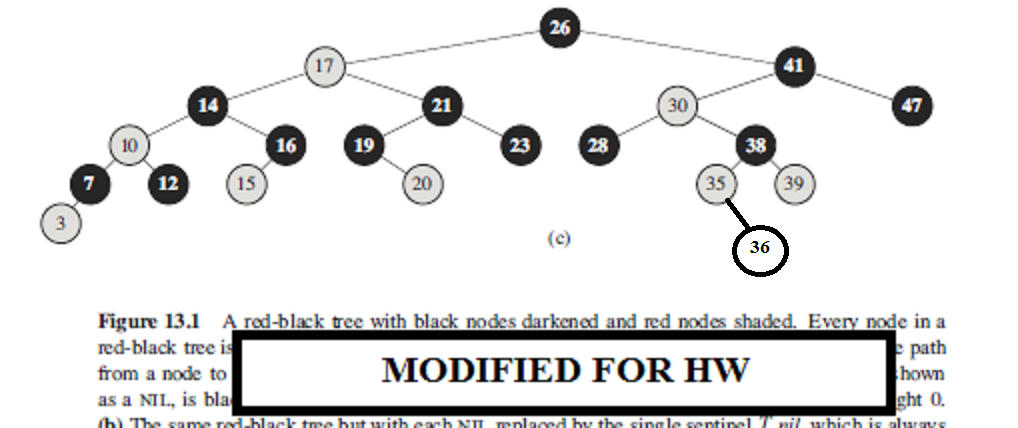
\includegraphics[width=1.0\textwidth]{Fig13_1_c.PNG}
    \caption{The addition of a node with key 36 to the tree of Figure 13.1.}
  \end{figure}

  Given that TREE-INSERT does not do anything to maintain
  any of the properties of a red-black, this insert case will not lead to a
  valid red-black tree. If the inserted node is red, then the resulting tree
  has two red nodes in a row, which is a violation of property \#4,
  if the inserted node is colored black, this is still not a valid red-black
  tree because the black-height of all subtrees will not be the same
  without rotations to even out the black heights, violating property \#5. \\

  %-----------------------------------------------------------------------------
  %-------     B     -----------------------------------------------------------
  %-----------------------------------------------------------------------------
  \item 13.1-3: Let us define a \textbf{relaxed red-black tree} as a binary
        search tree that satisfies redblack properties 1, 3, 4, and 5.
        In other words, the root may be either red or black. Consider a
        relaxed red-black tree $T$ whose root is red. If we color the root of
        $T$ black but make no other changes to $T$ , is the resulting tree
        a red black tree? \\

  \textbf{Solution:} Yes. Because property \#4 (if a node is red, both of its
  children must be black) is still maintained in the relaxed red-black
  in the red black tree, we can say that any children of the (red) root
  will be black. Changing the root to black will not violate properties \#1
  (each node will still be red or black), \#3 (every leaf (nil) will still
  be black), \#4 (any red nodes will still have black children), and \#5
  (the black heights at every node will be the dame for any of its
  sub-trees).


  \end{enumerate}

\newpage
%~~~~~~~~~~~~~~~~~~~~~~~~~~~~~~~~~~~~~~~~~~~~~~~~~~~~~~~~~~~~~~~~~~~~~~~~~~~~~~~
%~~~~~~~     Number 2     ~~~~~~~~~~~~~~~~~~~~~~~~~~~~~~~~~~~~~~~~~~~~~~~~~~~~~~
%~~~~~~~~~~~~~~~~~~~~~~~~~~~~~~~~~~~~~~~~~~~~~~~~~~~~~~~~~~~~~~~~~~~~~~~~~~~~~~~
\item Exercise 13.3-5 (page 322): Consider a red-black tree formed by
  inserting n nodes with
  RB-INSERT. Argue that if $n > 1$, the tree has at least one red node. \\

  \textbf{Solution:} I will make my argument using induction: \\

  \textit{Inductive hypothesis} \\
  The hypothesis is that inserting any number of nodes $n$, $\forall n > 1$,
  will leave at least one red node in the tree. \\

  \textit{Base Case} \\
  Inserting one node will result in that node being painted black to comply
  with property \#2 (the root must be black). Clearly, this does not result
  in at least one red node in the tree, so it cannot be our base case
  (which is fine, because we did not define our base case this way).
  The true base case involves the next
  node to be inserted (so actual base case is $n = 2$). This node will
  be inserted
  as a red node, and this node will not be re-painted or relocated because it
  is red or black (1), the root node will remain black (2), the leaves will
  remain black as long as the inserted red node is made to point to the NIL
  node as a child (3 and 4), and the new red node will not change the black
  height of any subtree (5), so since all properties hold, no changes
  need to be made. \\

  \textit{Assumption} \\
  Assume that inserting $n$ nodes will produce at least 1 red node in
  the tree. \\

  \textit{To Show} \\
  If an additional node is inserted, it will be inserted as red, and one of
  2 things can occur:
    \begin{itemize}
      \item The new node is inserted as the child of a black node. \\
      \item The new node is inserted as the child of a red node.
    \end{itemize}
  In the first case, inserting a red node will not alter/violate any of
  the 5 red-black tree properties, so no transformations to fix the tree
  will be made, leaving the red node in the tree, and the hypothesis holds.

  In the second case, transformations must be made to alter the tree to
  undo the violation of property \#4 so that no red node has a red child.
  There are 3 such transformations used to remedy 3 different cases of
  property violating insertions. The three transformations are:
    \begin{itemize}
      \item Node re-painting to "push a red node up the tree" \\
      \item A left rotation of a particular pair of nodes \\
      \item A right rotation of a perticular pair of nodes
    \end{itemize}
  The three cases where any of these transformations might be applied are:
    \begin{itemize}
      \item Case 1: When a red node is inserted as the child of a red node whose
            sibling is also red \\
      \item Case 2: When a red node is inserted as the child of a red node whose
            sibling is black \\
      \item Case 3: When a red node is inserted as the "inside"
            child of a red node whose sibling is black 
    \end{itemize}
    Note that of the three transformations, only a re-paint will alter the
    number of red nodes in the tree. This re-paint only occurs when "Case 1"
    appears, the case when a black parent node with two red children,
    and one red grandchild, is detected. In this case, the re-paint
    results in two red nodes
    (the children) and a black one (the parent) being exchanged for two blacks
    (again, the children) and a red one (the parent). The red grandchild
    is left unaltered. So even though the re-paint operation essentially
    merges two reds, there will still be two red nodes left after the operation.
    Even if the red node gets pushed up to become the root node and it
    gets repainted black, the red grandchild will still remain, so at least
    one red node (usually more) will always remain in a red-black tree
    with 2 or more nodes.

\newpage
%~~~~~~~~~~~~~~~~~~~~~~~~~~~~~~~~~~~~~~~~~~~~~~~~~~~~~~~~~~~~~~~~~~~~~~~~~~~~~~~
%~~~~~~~     Number 3     ~~~~~~~~~~~~~~~~~~~~~~~~~~~~~~~~~~~~~~~~~~~~~~~~~~~~~~
%~~~~~~~~~~~~~~~~~~~~~~~~~~~~~~~~~~~~~~~~~~~~~~~~~~~~~~~~~~~~~~~~~~~~~~~~~~~~~~~
\item Exercise 14.1-6 (page 345): Observe that whenever we
  reference the size attribute of a node in either OS-SELECT
  or OS-RANK, we use it only to compute a rank. Accordingly, suppose
  we store in each node its rank in the subtree of which it is
  the root. Show how to
  maintain this information during insertion and deletion.
  (Remember that these two
  operations can cause rotations.) \\

  \textbf{Solution:} In general, ranks can be adjusted as the tree is
  descended in the search for insertion/deletion points. Because rank
  information refers only to a node's rank within its sub-tree, not all
  ranks need to be updated every time the tree is altered. Each node's
  rank information depends only on the size of its right sub-tree. \\

  \textit{Insert} \\
  During insertion, as the tree is descended, if the search path needs to go
  right, then the current node's rank should be incremented before the search
  goes down the right path. Once the insertion point is found, the new node
  should be given a rank of 1. During fix-up, should a right rotation occur,
  then the node that was on the left (the one that will be rotated "upward")
  will need to be given a rank equal to the rank it originally had plus the
  rank of the right node (the one that is rotated "downward"), the size of the
  left node's right sub-tree. In a left rotation, the right node that is
  moved upward will keep it's rank. The left node that is moved downward will
  get a rank equal to its new right child's (the right node's former left
  child) rank plus one. \\

  \textit{Delete} \\
  When deleting a node in the modified OS-tree, when searching for the
  node to be deleted, as the search descends the tree to the right, the
  rank of the current node should be decremented before the search descends
  to the right, similar to the way ranks were incremented in the insertion
  process. The node to be deleted is either removed,
  or its in-order predecessor is removed in the same manner via recursion.
  This will work for all 3 deletion cases. Again, should a rotation occur, in
  the case that it is a right rotation, the left node will get the rank it had
  originally plus the right node's rank; the right node's rank will remain
  unchanged. In the case of a left rotation, the left node that is moved
  downward will receive a rank of its new right child plus one; the right
  node will keep the same rank it had originally because it's right sub-tree
  will not have changed.

\newpage
%~~~~~~~~~~~~~~~~~~~~~~~~~~~~~~~~~~~~~~~~~~~~~~~~~~~~~~~~~~~~~~~~~~~~~~~~~~~~~~~
%~~~~~~~     Number 4     ~~~~~~~~~~~~~~~~~~~~~~~~~~~~~~~~~~~~~~~~~~~~~~~~~~~~~~
%~~~~~~~~~~~~~~~~~~~~~~~~~~~~~~~~~~~~~~~~~~~~~~~~~~~~~~~~~~~~~~~~~~~~~~~~~~~~~~~
\item Exercise 14.3-3 (page 353): Describe an efficient algorithm that,
  given an interval $i$, returns an interval overlapping
  $i$ that has the minimum low endpoint, or $T.nil$
  if no such interval exists. \\

  \textbf{Solution:} An efficient algorithm that would accomplish this should
  ideally do so in \BigTheta{\lg{n}} time. Since interval trees are sorted by
  the low end point of their intervals, this could be accomplished by
  searching for an interval with that has a low value that overlaps with $i$,
  then by moving leftwards, down the tree to find the interval that still
  overlaps with interval $i$ but that has the lowest endpoint. Such an
  algorithm would look like:

  \begin{algorithm}{FIND-LOWEST-INTERVAL}[ T, i ]{}
%    \qcomment{}}
  $x \qlet T.root$ \\
  \qcom{Find the first overlapping interval} \\
  \qwhile $x \neq T.nil$ \qand ($i.high < x.low$) \qand ($i.low > x.high$) \\
  \qdo \\
    \qif $i.high < x.low$ \\
    \qthen \\
      $x \qlet x.right$ \\
    \qelse \\
      \qif $i.low > x.high$ \\
      \qthen
        $x \qlet x.left$
      \qfi
    \qfi
  \qelihw \\

  \qcom{Find the overlapping interval with the lowest end point} \\
  \qwhile $ x.left \neq T.nil$ \qand $i.high \ge x.low $ \\
    \qdo $x \qlet x.left$
  \qelihw \\

  \qcom{Return a pointer to the found node (or \qnil)} \\
  \qreturn $x$
  \end{algorithm}

  This algorithm is basically a modified binary search that spends constant
  time at each node, and only visits one node per level of the tree, so it
  intutitively is a \BigTheta{\lg{n}} algorithm.

\newpage
%~~~~~~~~~~~~~~~~~~~~~~~~~~~~~~~~~~~~~~~~~~~~~~~~~~~~~~~~~~~~~~~~~~~~~~~~~~~~~~~
%~~~~~~~     Number 5      ~~~~~~~~~~~~~~~~~~~~~~~~~~~~~~~~~~~~~~~~~~~~~~~~~~~~~
%~~~~~~~~~~~~~~~~~~~~~~~~~~~~~~~~~~~~~~~~~~~~~~~~~~~~~~~~~~~~~~~~~~~~~~~~~~~~~~~
\item Exercise 9.1-1 (page 215): Show that the second smallest of $n$
  elements can be found with $n + \lceil \lg{n} \rceil - 2$
  comparisons in the worst case. (\textit{Hint}: Also
  find the smallest element.) \\

  \textbf{Solution:} It is known that it takes $n - 1$ comparisons to find
  the smallest element in a set by conducting a "tournament" where elements
  are compared using a divide and conquer strategy. This method is often
  represented graphically using a tree. If an element "beats" another, it
  advances to a higher level of the tree to be compared to another element of
  the set, and the "losing" element is no longer compared to any
  other elements. It can be seen that $n - 1$ comparisons were made because
  a complete binary tree has at most $n - 1$ internal nodes (nodes that are
  not leaves). This is can be seen by solving the sum
  $\sum_{i=0}^{\lg{n}}{2^{i}} = 2n - 1$ which gives the number of
  all the nodes in a full binary tree, and then subtracting the $n$ leaves
  gives $n - 1$ remaining nodes (for a FULL binary tree). The number of
  internal nodes is significant because it counts the number of comparison
  results. For a less than full binary tree, there will be fewer comparisons
  because "byes" will appear in our tournament.

  The second smallest element would have lost to the smallest element somewhere
  in the tournament. The number of elements that were compared to the
  smallest element would be at most $\lceil \lg{n} \rceil$ elements,
  or one for each level of the
  the tree formed by the tournament (not counting the root level, where
  there are no more elements to compare with the smallest elemtent), since the 
  height of a complete binary tree is $\lceil \lg{n} \rceil + 1$.
  To find the second
  smallest element, one only needs to gather all the elements that were
  compared with the smallest element in the first tournament and hold a
  sort of "consolation" tournament. The winner of this second tournament will
  be the second smallest element of the set. Since it is known that holding
  a tournament with $n$ elements requires $n - 1$ comparisons (see above),
  then a tournament of $\lg{n}$ nodes would require $\lg{n} - 1$ comparisons.

  Thus, combining the costs of the tournaments results in
  $n - 1 + \lceil \lg{n} \lceil - 1 = n + \lceil \lg{n} \rceil - 2$
  comparisons.

  I feel is should be noted that while this algortithm might technically
  be optimal in terms of comparisons, it does invlove the overhead of storing
  lists of elements for the participant elements of the second tournament.
  This is not ideal if space is a concern. An "in-place" iterative algorithm
  would be ideal for space usage, and could perform the same operation in
  at most $2n -3$ comparisons, which is \BigO{n} time, similar to
  the algortithm above. But, since the question only asked about comparisons,
  I won't go in to this further.

\newpage
%~~~~~~~~~~~~~~~~~~~~~~~~~~~~~~~~~~~~~~~~~~~~~~~~~~~~~~~~~~~~~~~~~~~~~~~~~~~~~~~
%~~~~~~~     Number 6      ~~~~~~~~~~~~~~~~~~~~~~~~~~~~~~~~~~~~~~~~~~~~~~~~~~~~~
%~~~~~~~~~~~~~~~~~~~~~~~~~~~~~~~~~~~~~~~~~~~~~~~~~~~~~~~~~~~~~~~~~~~~~~~~~~~~~~~
\item Exercise 13.2-4 (page 314): Show that any arbitrary n-node
  binary search tree can be transformed into any other
  arbitrary n-node binary search tree using \BigO{n} rotations.
  (\textit{Hint}: First show that at most $n - 1$ right rotations
  suffice to transform the tree into a right-going chain.)\\

  \textbf{Solution:} Using the hint, consider how to turn any tree into a 
  right-going chain using at most $n - 1$ right rotations. If one were to use
  right rotations that were proximal to the \emph{right spine} of the tree,
  that is right rotations involving one node already in the right spine of
  the tree and one node exactly one leftward branch away from the spine.
  Each right rotation would move one node into the right spine and push the
  other node involved down a level in the right spine of the tree.
  The net result is that 1 node was moved into the right spine of the tree, and
  none were moved out of the right spine. If we were to consider the root
  node as already being in the right spine, then even in the worst case where
  the other $n - 1$ nodes are not in the right spine, they can be moved over
  one at a time.

  Let any sequence of right rotations that transform a binary tree to
  a right-going chain be denoted as $R_i$. Note that the effects of
  any rightward rotation can be reversed with a leftward rotation.
  Let a sequence that transforms a right-going chain back to an
  arbitrary binary tree by reversing the right rotations of sequence
  $R_i$ be denoted by $L_i$.

  Considering these two facts, suppose we have some arbitrarily constructed
  binary tree $T_1$. Then we can transform this tree into a right-going chain by
  shifting all of it's nodes into a right spine, call this sequence of
  rotations $R_1$. Now suppose we have a second tree, $T_2$, that can be
  transformed to a right-going chain by the sequence of right rotations $R_2$.
  Then we could transform $T_1$ to $T_2$ by applying rotation sequences
  $R_1$ and $L_2$, and vice versa. The size of each rotation sequence is at
  most $n - 1$, so even by fully using both rotation sequences, at most
  $2 * (n - 1) = 2n - 2$ rotations are performed, which, of course, is
  \BigO{n} rotations.

\end{enumerate}
%\LAST PAGE
\end{document}



%~~~~~~~~~~~~~~~~~~~~~~~~~~~~~~~~~~~~~~~~~~~~~~~~~~~~~~~~~~~~~~~~~~~~~~~~~~~~~~~
%~~~~~~~     Number 1     ~~~~~~~~~~~~~~~~~~~~~~~~~~~~~~~~~~~~~~~~~~~~~~~~~~~~~~
%~~~~~~~~~~~~~~~~~~~~~~~~~~~~~~~~~~~~~~~~~~~~~~~~~~~~~~~~~~~~~~~~~~~~~~~~~~~~~~~
\item Implement a Max algorithm (in C/C++) that uses a divide and conquer
strategy to find the maximum among N items stored in an array
A[0], \dots, A[n-1]. To illustrate the sequence of function calls made
by your algorithm, each call to the algorithm should print the
following tuple: \textless Return-Value, "Max(left-idx,
right-idx)" \textgreater where Return-Value
is the maximum value returned by that call and left-idx and
right-idx are the indices of the array with which that particular
recursive call is made.

  \begin{enumerate}
  %-----------------------------------------------------------------------------
  %-------     A     -----------------------------------------------------------
  %-----------------------------------------------------------------------------
  \item Submit your code for the algorithm. \\

  \textbf{Solution:}
    \begin{verbatim}
template <typename ItemType>
ItemType Max( ItemType* A, unsigned int left_idx, unsigned int right_idx )
{
  // variables
  ItemType Return_Value;
  ItemType left_temp;
  ItemType right_temp;
  int current_array_size = ( right_idx - left_idx + 1 );
  int left_upper_bound = 0;
  int right_lower_bound = 0;

  // base case: the current sub_array size is less than or equal to 2
  if( current_array_size == 1 )
  {
    // the only item is the greatest item
    Return_Value = A[left_idx];
  }
  // case: the current sub_array size is greater than 2
  else
  {
    // find the boundary indices of the two sub-arrays
    left_upper_bound = ( left_idx + right_idx ) / 2;
    right_lower_bound = ( ( left_idx + right_idx ) / 2 ) + 1;

    // find the max of each sub_array
    left_temp = Max( A, left_idx, left_upper_bound );
    right_temp = Max( A, right_lower_bound, right_idx );

    // find the greater of the two values
    Return_Value = ( left_temp < right_temp ? right_temp : left_temp );
  }

  // state the effect of this action for homework proposes
  cout << "<" << Return_Value << ", Max(" << left_idx << ", " << right_idx
       << ")>" << endl;

  // return the maximum value found for this array/sub-array
  return Return_Value;
}
    \end{verbatim}
\newpage

  %-----------------------------------------------------------------------------
  %-------     B     -----------------------------------------------------------
  %-----------------------------------------------------------------------------
  \item Submit the analysis of the running time of your algorithm. \\

  \textbf{Solution:} The running time for this algorithm can be summarized by
  the following table: \\
    \begin{center}
    \begin{tabular}{| c || c | c |}
      \hline
      Step Number & Action & Times Executed  \\
      \hline \hline
      1.          & Variable initialization and computation & $1$ \\
      \hline
      2.          & Compare the array size & $1$ \\
      \hline
      3.          & In the base case, make an assignment & $1$ \\
      \hline
      4.          & In the other case, compute the sub-array
                    bounds                                   & \BigTheta{1} \\
      \hline
      5.          & Make 2 recursive calls to find the
                    max of each sub-array              & $2 * M(\frac{n}{2})$ \\
      \hline
      6.          & Compare/assign the max of the two
                    sub-arrays                         & $1$ \\
      \hline
      7.          & Return the maximum value found     & $1$ \\
      \hline
    \end{tabular}
    \end{center}

    So it would be reasonable to say that in general this algorithm is
    representedby the recurrence: 
    \[ M(n) = 2 * M(\frac{n}{2}) + \BigTheta{1} \]
    and even more accurately by:
    \begin{equation*}
    M(x) = \left\{
          \begin{array}{rl}
          \BigTheta{1}                             & \text{if } n = 1 \\
          M(n) = 2 * M(\frac{n}{2}) + \BigTheta{1} & \text{if } n > 1
          \end{array} \right.
    \end{equation*}
    Using the "Recursion Tree" method, we can see that the problem size at
    each node will be $\frac{n}{2^{i}}$, with a constant cost at each level;
    $1 = \frac{n}{2^{i}}$
    gives $i = \lg{n}$, where $i$ is the number of recursive calls made.
    Note that at each level, the number of nodes at level $i$ is $2^i$ for
    this algortihm.
    So, summing the cost of all levels but the last one, and then adding
    the cost of the lowest level/leaves gives:
    \begin{align*}
      M(n) &= \sum_{i=0}^{\lg{n}}{1} + 2^{\lg{n}}M(1) \\
           &= \lg{n} + n * M(1) \\
           &= \BigTheta{\lg{n}} + n \\
           &= \BigTheta{\lg{n}} + \BigTheta{n} \\
      M(n) &= \BigTheta{n}
    \end{align*}

\newpage
  %-----------------------------------------------------------------------------
  %-------     C     -----------------------------------------------------------
  %-----------------------------------------------------------------------------
  \item Submit the output of your algorithm for the following input: \\
        A = [ T I N Y E X A M P L E ] \\

  \textbf{Solution:}
    \begin{verbatim}
Testing Problem 1 code by outputting
<Return_Value, Max(left_idx, right_idx)> tuples
=======================================================
<T, Max(0, 0)>
<I, Max(1, 1)>
<T, Max(0, 1)>
<N, Max(2, 2)>
<T, Max(0, 2)>
<Y, Max(3, 3)>
<E, Max(4, 4)>
<Y, Max(3, 4)>
<X, Max(5, 5)>
<Y, Max(3, 5)>
<Y, Max(0, 5)>
<A, Max(6, 6)>
<M, Max(7, 7)>
<M, Max(6, 7)>
<P, Max(8, 8)>
<P, Max(6, 8)>
<L, Max(9, 9)>
<E, Max(10, 10)>
<L, Max(9, 10)>
<P, Max(6, 10)>
<Y, Max(0, 10)>
    \end{verbatim}

  \end{enumerate}

\newpage
%~~~~~~~~~~~~~~~~~~~~~~~~~~~~~~~~~~~~~~~~~~~~~~~~~~~~~~~~~~~~~~~~~~~~~~~~~~~~~~~
%~~~~~~~     Number 2     ~~~~~~~~~~~~~~~~~~~~~~~~~~~~~~~~~~~~~~~~~~~~~~~~~~~~~~
%~~~~~~~~~~~~~~~~~~~~~~~~~~~~~~~~~~~~~~~~~~~~~~~~~~~~~~~~~~~~~~~~~~~~~~~~~~~~~~~
\item Implement a bottom-up Mergesort algorithm (in C/C++) that works by
      making a sequence of passes over the entire array doing m-by-m merges,
      doubling m on each pass. For example, the algorithm first scans
      through the input performing 1-by-1 merges ot produce ordered
      sub-arrays of size 2; then, it scans through the input again performing
      2-by-2 merges to produce ordered sub-arrays of size 4, and so on until
      the entire array is sorted. At each call to Merge, print out the input
      array that is being processed by that function call. Note: the final
      Merge may be an m-by-x merge, for some x less than or equal to m
      (if the array size is a multiple of m).

  \begin{enumerate}
  %-----------------------------------------------------------------------------
  %-------     A     -----------------------------------------------------------
  %-----------------------------------------------------------------------------
  \item Submit your code for the algorithm. \\

  \textbf{Solution:} (Note: \textit{Merge} code adapted from
          lecture notes/textbook)
  \begin{verbatim}
template <typename ItemType>
void bottomUpMergeSort( ItemType* A, int n )
{
  // variables
  int m = 1; // the sub-array size to merge into size 2m
  int right_start = 0;
  int right_end = 0;
  int left_end = 0;

  // scan array, performing merges until two sub-arrays have been merged
  // to the original size
  while( m < n )
  {
    // perform the merge-scanning for the current sub-array size
    for( right_start = 0; right_start < n; right_start += ( 2 * m ) )
    {
      // find the end of the right sub-array
      right_end = right_start + m - 1;

      // find the end of the sub_arrays combined
      left_end = right_end + m;
      if( left_end >= n )
      {
        // prevent the end marker for the sub-arrays from overreaching the array
        left_end = n - 1;
      }

      // merge each pair of sub-arrays
      Merge( A, right_start, right_end, left_end );
    }

    // move up to the next sub-array size
    m *= 2;
  }

  // no return - void
}


template <typename ItemType>
void Merge( ItemType* A, int p, int q, int r )
{
  // variables
  int main_ndx = p;
  int left_ndx = 0;
  int right_ndx = 0;
  int left_size = q - p + 1;
  int right_size  = r - q;
  ItemType temp;
  ItemType left_array[left_size + 1];
    left_array[left_size] = kSentinel;
  ItemType right_array[right_size + 1];
    right_array[right_size] = kSentinel;

  // print the array being processed for hw purposes
  cout << "p: " << p << ", q: " << q << ", r: " << r << endl;
  cout << "Before: ";
  for( main_ndx = p; main_ndx <= r; main_ndx++ )
  {
    cout << A[main_ndx] << ' ';
  }
  cout << endl;

  // load up the sub-arrays
  for( main_ndx = p, left_ndx = 0; main_ndx <= q; left_ndx++, main_ndx++ )
  {
    // copy the element over
    left_array[left_ndx] = A[main_ndx];
  }
  for( right_ndx = 0; main_ndx <= r; right_ndx++, main_ndx++ )
  {
    // copy the element over
    right_array[right_ndx] = A[main_ndx];
  }


  // perform the merging
  for( main_ndx = p, right_ndx = 0, left_ndx = 0; main_ndx <= r; main_ndx++ )
  {
    // case: the element of the left sub-array is less or equal
    if( left_array[left_ndx] <= right_array[right_ndx] )
    {
      // store the element in the original array
      A[main_ndx] = left_array[left_ndx];

      // move on to the next element of the right sub-array
      left_ndx++;
    }
    // case: the item in the right array is the lesser of the two elements
    else
    {
      // store the element in the original array
      A[main_ndx] = right_array[right_ndx];

      // move on to the next element of the right sub-array
      right_ndx++;
    }
  }

  // print the merge result for hw purposes
  cout << "After:  ";
  for( main_ndx = p; main_ndx <= r; main_ndx++ )
  {
    cout << A[main_ndx] << ' ';
  }
  cout << endl << endl;

  // no return - void
}
  \end{verbatim}

  %-----------------------------------------------------------------------------
  %-------     B     -----------------------------------------------------------
  %-----------------------------------------------------------------------------
  \item Submit the output of your algorithm for the following input: \\
        A = [ A S O R T I N G E X A M P L E ] \\

  \textbf{Solution:}
  \begin{verbatim}
Testing Problem 2 code by outputting
the sub-arrays to be processed
=======================================================
p: 0, q: 0, r: 1
Before: A S 
After:  A S 

p: 2, q: 2, r: 3
Before: O R 
After:  O R 

p: 4, q: 4, r: 5
Before: T I 
After:  I T 

p: 6, q: 6, r: 7
Before: N G 
After:  G N 

p: 8, q: 8, r: 9
Before: E X 
After:  E X 

p: 10, q: 10, r: 11
Before: A M 
After:  A M 

p: 12, q: 12, r: 13
Before: P L 
After:  L P 

p: 14, q: 14, r: 14
Before: E 
After:  E 

p: 0, q: 1, r: 3
Before: A S O R 
After:  A O R S 

p: 4, q: 5, r: 7
Before: I T G N 
After:  G I N T 

p: 8, q: 9, r: 11
Before: E X A M 
After:  A E M X 

p: 12, q: 13, r: 14
Before: L P E 
After:  E L P 

p: 0, q: 3, r: 7
Before: A O R S G I N T 
After:  A G I N O R S T 

p: 8, q: 11, r: 14
Before: A E M X E L P 
After:  A E E L M P X 

p: 0, q: 7, r: 14
Before: A G I N O R S T A E E L M P X 
After:  A A E E G I L M N O P R S T X 
  \end{verbatim}

  \end{enumerate}

\newpage
%~~~~~~~~~~~~~~~~~~~~~~~~~~~~~~~~~~~~~~~~~~~~~~~~~~~~~~~~~~~~~~~~~~~~~~~~~~~~~~~
%~~~~~~~     Number 3     ~~~~~~~~~~~~~~~~~~~~~~~~~~~~~~~~~~~~~~~~~~~~~~~~~~~~~~
%~~~~~~~~~~~~~~~~~~~~~~~~~~~~~~~~~~~~~~~~~~~~~~~~~~~~~~~~~~~~~~~~~~~~~~~~~~~~~~~
\item Does the Merge procedure produce proper output if and only if the two
      input sub-arrays are in sorted order? Prove your answer, or provide a
      counterexample. \\

  \textbf{Solution:} In order to prove this, we first need to prove that Merge
  works if the sub-arrays are sorted, and will not work if they are not
  properly sorted.\\

  \textit{Merge works if sub-arrays are sorted.}\\

  \underline{Invariant}: The \emph{output array} will always remain sorted;
  any elements remaining in the \emph{sub-arrays} will be sorted and
  greater than any elements in the output array.\\

  \underline{Initialization}: When the two sub-arrays are untouched and the
  \emph{output array} is empty, then the output array is sorted because there
  are no contents to be disordered. Similarly, if only one element has been
  taken from either of the sub-arrays (the least element of the two) and
  placed in the output array, we consider this one element to be sorted; of
  course the sub-array is sorted.\\

  \underline{Maintenance}: If items are taken from the sub-arrays one at a
  time, taking the least next remaining element of the two, and adding it to the
  output array, then the output array remains sorted. Any element still
  remaining in the sub-arrays must be greater than any element that was taken
  before it (due to our assumption that the sub-arrays are sorted), along
  with only taking the least available element ensures that
  the ouput array will not have been disordered. Taking
  only the next remaining element (which will be the least remaining)
  cannot disorder a sub-array.\\

  \underline{Termination}: Once both sub-arrays are empty, they are still
  "sorted." The output array must be sorted (see the Maintenance
  Condition), an so upon termination, the output is both complete and sorted. \\

  \textit{Merge does not work if sub arrays are not sorted.}\\

  Assume that Merge still works with unsorted sub-arrays.
  Consider a case where the sub-arrays' first available element is not sorted,
  but their second available element is their least element. The remaining
  elements can be in any order. As items are transferred to the output array,
  the first items are taken, but then once the second/least elements are
  reached and placed in the output array, the output array is instantly
  unsorted. A constradiction has arisen, so we know that only having sorted
  sub-arrays enables Merge success.\\

  Thus, the Merge procedure produces proper output if and only if the
  sub-arrays are sorted.

\newpage
%~~~~~~~~~~~~~~~~~~~~~~~~~~~~~~~~~~~~~~~~~~~~~~~~~~~~~~~~~~~~~~~~~~~~~~~~~~~~~~~
%~~~~~~~     Number 4     ~~~~~~~~~~~~~~~~~~~~~~~~~~~~~~~~~~~~~~~~~~~~~~~~~~~~~~
%~~~~~~~~~~~~~~~~~~~~~~~~~~~~~~~~~~~~~~~~~~~~~~~~~~~~~~~~~~~~~~~~~~~~~~~~~~~~~~~
\item For sort, in situations where there are large numbers of
duplicate keys in the unput file, there is potential for significant
improvement of the algorithm. One solution is to partition the file into
\textbf{three} parts, one each for keys \textit{smaller than},
\textit{equal to} and \textit{larger than} the partitioning element. In
this approach the keys equal to the partitioning element that are
encountered in the left partition are kept at the partition's left end and
the keys equal to the partitioning element that are encountered in the
right partition are kept at the partition's right end. \textbf{Implement}
in C/C++ this partitioning strategy as follows: choose the pivot to be the
last element of the array. Scan the file from the left to find an element
that is not smaller than the partitioning element and from the right to
find an element that is not larger than the partitioning element, then
exchange them. If the element on the left (after the exchange) is equal
to the partitioning element, exchange it with the one at the left end of
the partition (similarly on the right). When the pointers cross, put the
partitioning element between the two partitions, then exchange all the
keys equal to it into position on either side of it (the figure on the
right (not shown) illustrates this process. During partitioning the
algorithm maintains the following situation:
\begin{center}
\begin{tabular}{|c|c|c|c|c|c|}
  \hline
  equal & less & XXX & greater & equal & v \\
  \hline
\end{tabular}
\end{center}
(indices/pointers not shown)\\
Illustrate the behavior of your algorithm on the input in the above
figure by printing, after each iteration (left \& right scan and
eventual changes), the elements in the partitions as in the example
above (not shown).\\

  \begin{enumerate}
  %-----------------------------------------------------------------------------
  %-------     A     -----------------------------------------------------------
  %-----------------------------------------------------------------------------
  \item Submit your code for the algorithm. \\

  \textbf{Solution:}
  \begin{verbatim}
template <typename ItemType>
void threePartQuicksort( ItemType* A, int partition_start, int partition_end )
{
  // variables
  int pivot_ndx = partition_end - 1;
  int left_ndx = partition_start;
  int right_ndx = pivot_ndx - 1;
  int left_equal_ndx = left_ndx;
  int right_equal_ndx = right_ndx;
  ItemType pivot = A[pivot_ndx];

  // output the array for hw purposes
  cout << "At the start of a new call:" << endl;
  arrayPrint( A, partition_start, left_equal_ndx, left_ndx,
              right_ndx, right_equal_ndx, pivot_ndx );

  // case: the partition size is larger than 1
  if( partition_start < pivot_ndx )
  {
    // perform scanning and swapping to create the left and right partitions
    while( left_ndx < right_ndx )
    {
      // swap the two items to correctly partition them
      swap( A[left_ndx], A[right_ndx] );

      // case: the item at the left index is equal to the pivot
      //       and there is a not-equal element to swap it with
      if( ( A[left_ndx] == pivot ) && ( left_equal_ndx < left_ndx ) )
      {
        // make the swap
        swap( A[left_ndx], A[left_equal_ndx] );

        // update the left-equal sub-partition and the left partition
        left_equal_ndx++;
        left_ndx++;
      }

      // case: the item at the right index is equal to the pivot
      //       and there is a-not equal element to swap it with
      if( ( A[right_ndx] == pivot ) && ( right_ndx < right_equal_ndx ) )
      {
        // make the swap
        swap( A[right_ndx], A[right_equal_ndx] );

        // update the right-equal sub-partition and the right partition
        right_equal_ndx--;
        right_ndx--;
      }

      // scan from the left for an element that is not less than the pivot
      while( ( A[left_ndx] < pivot ) && ( left_ndx < pivot_ndx ) )
      {
        // advance the left index
        left_ndx++;
      }

      // scan from the right for an element that is not greater than the pivot
      while( ( A[right_ndx] > pivot ) && ( right_ndx > partition_start ) )
      {
        // advance the left index
        right_ndx--;
      }

      // output the array for hw purposes
      cout << "After an iteration of scan/swapping:" << endl;
      arrayPrint( A, partition_start, left_equal_ndx, left_ndx,
                  right_ndx, right_equal_ndx, pivot_ndx );
    }

    // case: the pivot is greater than all other elements in the partition
    //       (no left partition can/should be made)
    if( left_ndx < pivot_ndx )
    {
      // move the pivot to create 3 partitions: right, middle, left
      swap( A[left_ndx], A[pivot_ndx] );
      right_ndx = left_ndx - 1;
      left_ndx++;

      // bump everything from the left-equal sub-partition to the middle
      while( left_equal_ndx > partition_start )
      {
        left_equal_ndx--;
        swap( A[left_equal_ndx], A[right_ndx] );
        right_ndx--;
      }

      // bump everything from the right-equal sub-partition to the middle
      while( right_equal_ndx < pivot_ndx )
      {
        right_equal_ndx++;
        swap( A[right_equal_ndx], A[left_ndx] );
        left_ndx++;
      }
    }

    // display the effects of this function call for homework purposes
    cout << "After pivot swapping and creating the middle partition:" << endl;
    arrayPrint( A, partition_start, left_equal_ndx, left_ndx,
                right_ndx, right_equal_ndx, pivot_ndx );

    // sort the left partition
    threePartQuicksort( A, partition_start, right_ndx + 1 );

    // sort the right partition
    threePartQuicksort( A, left_ndx - 1, partition_end );
  }
  // base case: the partition was of size 1 or less
    // do nothing

  // display the effects of this function call for homework purposes
  cout << "At the end of a call:" << endl;
  arrayPrint( A, partition_start, left_equal_ndx, left_ndx,
              right_ndx, right_equal_ndx, pivot_ndx );

  // no return - void
}
  \end{verbatim}

\newpage
  %-----------------------------------------------------------------------------
  %-------     B     -----------------------------------------------------------
  %-----------------------------------------------------------------------------
  \item Submit the output of your algorithm for the following input: \\
        A = [ A B R A C A C A B R A B C D C ] \\

  \textbf{Solution:}
  \begin{verbatim}
Testing Problem 4 code by outputting
the array with various indices shown
=======================================================
At the start of a new call:
ABRACACABRABCDC
^            ^^
l            jr

After an iteration of scan/swapping:
DBRACACABRABCAC
^            ^^
l            jr

After an iteration of scan/swapping:
ABRACACABRABCDC
^ ^         ^^^
l i         jqr

After an iteration of scan/swapping:
CBAACACABRABRDC
^^  ^      ^ ^^
lp  i      j qr

After an iteration of scan/swapping:
CBAABACABRADRCC
^^    ^   ^ ^ ^
lp    i   j q r

After an iteration of scan/swapping:
CBAABAAABRRDCCC
^^      ^^ ^  ^
lp      ji q  r

After pivot swapping and creating the middle partition:
BBAABAAACCCCRDR
^      ^     ^^
l      j     ir

At the start of a new call:
BBAABAAA
^     ^^
l     jr

After an iteration of scan/swapping:
ABAABABA
^    ^^^
l    jqr

After an iteration of scan/swapping:
ABAABBAA
^  ^ ^ ^
l  j q r

After an iteration of scan/swapping:
ABABBAAA
^ ^ ^  ^
l j q  r

After an iteration of scan/swapping:
ABBBAAAA
^  ^   ^
l  q   r

After pivot swapping and creating the middle partition:
AAAAABBB
^    ^ ^
l    i r

At the start of a new call:




At the end of a call:




At the start of a new call:
    ABBB
    ^ ^^
    l jr

After an iteration of scan/swapping:
    BBAB
    ^ ^^
    l jr

After an iteration of scan/swapping:
    ABBB
    ^^^^
    lijr

After an iteration of scan/swapping:
    BABB
    ^^^^
    lpir

After pivot swapping and creating the middle partition:
    ABBB
    ^  ^
    l  r

At the start of a new call:
    A
    ^
    r

At the end of a call:
    A
    ^
    r

At the start of a new call:
       B
       ^
       r

At the end of a call:
       B
       ^
       r

At the end of a call:
    ABBB
    ^  ^
    l  r

At the end of a call:
AAAAABBB
^    ^ ^
l    i r

At the start of a new call:
            RDR
            ^^^
            ljr

After an iteration of scan/swapping:
            DRR
            ^^^
            lir

After pivot swapping and creating the middle partition:
            DRR
            ^ ^
            l r

At the start of a new call:
            D
            ^
            r

At the end of a call:
            D
            ^
            r

At the start of a new call:
              R
              ^
              r

At the end of a call:
              R
              ^
              r

At the end of a call:
            DRR
            ^ ^
            l r

At the end of a call:
AAAAABBBCCCCDRR
^      ^     ^^
l      j     ir
  \end{verbatim}
  \end{enumerate}

\newpage
%~~~~~~~~~~~~~~~~~~~~~~~~~~~~~~~~~~~~~~~~~~~~~~~~~~~~~~~~~~~~~~~~~~~~~~~~~~~~~~~
%~~~~~~~     Number 5      ~~~~~~~~~~~~~~~~~~~~~~~~~~~~~~~~~~~~~~~~~~~~~~~~~~~~~
%~~~~~~~~~~~~~~~~~~~~~~~~~~~~~~~~~~~~~~~~~~~~~~~~~~~~~~~~~~~~~~~~~~~~~~~~~~~~~~~
\item Problem 7-2 (page 186), parts (a), (c), and (d). For (c) and (d)
      assume that you have the procedure at point (b) available. \\
      \textbf{\textit{ Quicksort with equal element values }} \\
      The analysis of the expected running time of randomized quicksort in
      Section 7.4.2 assumes that all element values are distinct. In this
      problem, we examine what happens when they are not. \\
%!!!!!!!!!!!!!!!!!!!!!!!!!!!!!!!!!!!!!!!!!!!!!!!!!!!!!!!!!!!!!
% This problem was extra credit and I felt the questions were unclear,
% so these are NOT trustworthy answers
%!!!!!!!!!!!!!!!!!!!!!!!!!!!!!!!!!!!!!!!!!!!!!!!!!!!!!!!!!!!!!
  \begin{enumerate}
  %-----------------------------------------------------------------------------
  %-------     A     -----------------------------------------------------------
  %-----------------------------------------------------------------------------
  \item Suppose that all the element values are equal. What would be
        randomized quicksort's running time in this case? \\

  \textbf{Solution:} In this case, the partitioning would not really occur.
  Since no elements would be greater than any pivot, no left partition
  could ever be formed. With no left partition ever forming, the problem size
  could only decrease by one element. In determining that only one
  element could be reduced from the problem, all other elements had to
  be visited. Thus, we get:
  \begin{align*}
    Quicksort(n) &= \sum_{i=0}^{n-1}{n-i} \\
                 &= \frac{n^{2}+n}{2} \\
    Quicksort(n) &= \BigTheta{n^{2}}
  \end{align*}

  %-----------------------------------------------------------------------------
  %-------     B     -----------------------------------------------------------
  %-----------------------------------------------------------------------------
  \item \textbf{Not assigned.} \\
  The PARTITION procedure returns an index $q$ such that each element of
  A[$p \dots q - 1$] is less than or equal to A[$q$] and each element
  of A[$q + 1$ \dots $r$] is greater than $q$. Modify the
  PARTITION procedure to produce a procedure
  PARTITION'[A, $p$, $r$], which permutes the elements
  of A[$p \dots r$] and returns two
  indices $q$ and $t$, where $p \le q \le t \le r$,
  such that
  \begin{itemize}
    \item all elements of A[$q \dots t$] are equal, \\
    \item each element of A[$p \dots q - 1$] is less than A[$q$], and \\
    \item each element of A[$t + 1 \dots r$] is greater than A[$q$].
  \end{itemize}
  Like PARTITION, your PARTITION' procedure should
  take \BigTheta{r - p} time. \\


  %-----------------------------------------------------------------------------
  %-------     C     -----------------------------------------------------------
  %-----------------------------------------------------------------------------
  \item Modify the RANDOMIZED-QUICKSORT procedure to call PARTITION', and
        call the new procedure RANDOMIZED-QUICKSORT'. Then modify the
        QUICKSORT procedure to produce a procedure QUICKSORT'(p, r) that
        calls RANDOMIZED-PARTITION' and recurses only on partitions of
        elements not known to be equal to each other. \\

  \textbf{Solution:}
  \begin{algorithm}{RANDOMIZED-QUICKSORT'}[ A( 0 \dots n-1 ), p, r ]{
    \qcomment{// Input: an array A[0 \dots n-1, 0 \dots n-1]
                        of integer numbers} }
  \qif{p $<$ r} \\
    q, t = \text{RANDOMIZED-PARTITION'}(A, p , r) \qcomment{Two returns}\\
    RANDOMIZED-QUICKSORT'(A, p, q-1) \\
    RANDOMIZED-QUICKSORT'(A, t+1, r) \\
  \qfi
  \end{algorithm}

\newpage
  \begin{algorithm}{QUICKSORT'}[ A( 0 \dots n-1 ), p, r ]{
    \qcomment{// Input: an array A[0 \dots n-1, 0 \dots n-1]
                        of integer numbers} }
  \qif{p $<$ r} \\
    q, t = \text{RANDOMIZED-PARTITION'}(A, p , r) \qcomment{Two returns} \\
    RANDOMIZED-QUICKSORT'(A, p, q-1) \\
    RANDOMIZED-QUICKSORT'(A, t+1, r) \\
  \qfi 
  \end{algorithm}

  %-----------------------------------------------------------------------------
  %-------     D     -----------------------------------------------------------
  %-----------------------------------------------------------------------------
  \item Using QUICKSORT', how would you adjust the analysis in 7.4.2
        to avoid the assumption that all elements are distinct? \\

  \textbf{Solution:} Because the PARTITION' procedure groups all of the
  elements with the same value of the pivot, the problem size is decreased
  by faster than typical quicksort. We can avoid the assumption that all
  elements are distinct by simply not assuming that all elements are
  distinct. Then, in the case that some elements are the same, our problem size
  is decreased by more than 1 with each recursive call. There is still
  a problem size perhaps less than $n$ at each level of the tree, but there is
  still \BigTheta{n} work at each level. The height of this tree will be
  \BigTheta{\log_{3}{n}}, which is essentially \BigTheta{\lg{n}}. While the
  asymptotic notation may not show it, the new procedure will have a better
  time complexity in what would be the original QUICKSORT's worst case,
  but a worse time complexity if all of the elements are distinct.

  \end{enumerate}

\end{enumerate}
%\LAST PAGE
\end{document}























Consider the following algorithm:
\begin{algorithm}{Enigma}[ A( 0 \dots n-1, 0 \dots n-1 ) ]{
  \qcomment{// Input: a matrix A[0 \dots n-1, 0 \dots n-1] of integer numbers} }
\qfor{ $i \qlet 0$ \qto $n - 2$ } \\
\do \\
  \qfor{ $j \qlet i + 1$ \qto $n - 1 $ } \\
  \do \\
    \qif{ $ A[i, j] \ne A[j, i] $ } \\
      \qreturn \qfalse \qfi \qrof \qrof \\
\qreturn \qtrue
\end{algorithm}

  \begin{enumerate}
  %-----------------------------------------------------------------------------
  %-------     A     -----------------------------------------------------------
  %-----------------------------------------------------------------------------
  \item What does this algorithm do? \\

  \textbf{Solution:} This algorithm checks to see if all of the elements
  below the main diagonal of the matrix are equal to the element that
  is transposed from the
  original element in a matrix, i.e. symmetric about, but not including,
  the diagonal. If the matrix is symmetric in this manner, this is indicated
  by the returning of true after checking all the elements. If any pair of
  elements are detected to be asymmetric, the check halts and false is
  returned. \\

  %-----------------------------------------------------------------------------
  %-------     B     -----------------------------------------------------------
  %-----------------------------------------------------------------------------
  \item Compute the running time of this algorithm. \\

  \textbf{Solution:} Outline the number of times each primitive operation
  (primitive math operations, comparisons, etc.) occurs, consider primitive
  operations to have constant running time. Note that $t_x$ indicates the
  number of times a statement is executed for a given value of $x$. Then sum
  the cost multiples to get the running time of the algorithm. \\

  \textit{ Numbers refer to the steps of the algorithm above.}
    \begin{center}
    \begin{tabular}{| c || c | c | c |}
      \hline
      Step Number & Cost & Times Executed (Best Case)
          & Times Executed (Worst Case)  \\
      \hline \hline
      1.          & $c_1$  & $1$ & $\sum_{i=0}^{n-2}{1} = n - 1$  \\
      \hline
      2.          & $c_2$  & $1$ & $\sum_{i=0}^{n-2}{t_i} $ \\
      \hline
      3.          & $c_3$  & $1$ & $\sum_{i=0}^{n-2}{t_i - 1}$  \\
      \hline
      4.          & $c_4$  & $1$ & $0$  \\
      \hline
      5.          & $c_5$  & $0$ & $1$  \\
      \hline
    \end{tabular}
    \end{center}

  In the "best" case scenario, the very first pair of elements A[$i,j$] and
  A[$j,i$] are not equal, thus the first for-loop check will only execute once,
  the inner for-loop check will only execute once, and the if statement will
  only execute once, and of course the return statement will return once.
  In this case, $t_i = 1$, but this will make little difference overall:
  \begin{align*}
    T(n) &= c_1(1) + c_2(1) + c_3(1) + c_4(1) + c_5(0) \\
         &= c_1 + c_2 + c_3 + c_4 \\
         &= c_a \text{(an arbitrary constant)} \\
         &= \BigTheta{1}
  \end{align*}
%  In the "best" case, this function is \BigTheta{1}.
\newpage
  In the "worst" case, both loops will execute the maximum number of times
  because each pair of elements tested will be checked before true is
  finally returned.
  In this case the value for $t_i$ will be:
  \begin{align*}
    t_i &= \sum_{j=i+1}^{n-1}{1} \\
        &= ((n - 1) - (i + 1)) + 1 \\
        &= (n - i - 2) + 1 \\
        &= n - i - 1
  \end{align*}

  So the resulting time cost is:
  \begin{align*}
    T(n) &= c_1(\sum_{i=0}^{n-2}{1}) + c_2(\sum_{i=0}^{n-2}{t_i}) +
            c_3(\sum_{i=0}^{n-2}{t_i - 1}) + c_4(0) + c_5(1) \\
         &= c_1(n - 1) + c_2(\sum_{i=0}^{n-2}{n - i - 1}) +
            c_3(\sum_{i=0}^{n-2}{(n - i - 1) - 1}) + c_5 \\
         &= c_1(n - 1) +
            c_2(\sum_{i=0}^{n-2}{n}-\sum_{i=0}^{n-2}{i}-\sum_{i=0}^{n-2}{1}) +
            c_3(\sum_{i=0}^{n-2}{n - i - 2}) + c_5 \\
         &= c_1(n - 1) +
            c_2((n - 1)(n) - (\frac{(n-1)n}{2}) - (n - 1)) +
            c_3(\sum_{i=0}^{n-2}{n}-\sum_{i=0}^{n-2}{i}-\sum_{i=0}^{n-2}{2}) +
            c_5 \\
         &= c_1(n - 1) + c_2((n^{2} - n) - (\frac{n^{2} - n}{2}) - (n - 1)) +
            c_3((n - 1)(n) - (\frac{(n-1)n}{2}) - 2(n - 1)) + c_5 \\
         &= c_1(n - 1) + c_2(\frac{n^{2} - n}{2} - (n - 1)) +
            c_3(\frac{n^{2} - n}{2} - (2n - 2)) + c_5 \\
         &= c_1(n - 1) + c_2(\frac{n^{2} - 3n + 2}{2}) +
            c_3(\frac{n^{2} - 5n + 4}{2}) + c_5 \\
         &= an^{2} + bn + c \text{, for sufficient a, b, c} \\
         &= \BigTheta{n^{2}}
  \end{align*}
  \end{enumerate}
\newpage

%~~~~~~~~~~~~~~~~~~~~~~~~~~~~~~~~~~~~~~~~~~~~~~~~~~~~~~~~~~~~~~~~~~~~~~~~~~~~~~~
%~~~~~~~     Number 2     ~~~~~~~~~~~~~~~~~~~~~~~~~~~~~~~~~~~~~~~~~~~~~~~~~~~~~~
%~~~~~~~~~~~~~~~~~~~~~~~~~~~~~~~~~~~~~~~~~~~~~~~~~~~~~~~~~~~~~~~~~~~~~~~~~~~~~~~
\item Solve the following recurrences using a method of your choice:
  \begin{enumerate}
  %-----------------------------------------------------------------------------
  %-------     A     -----------------------------------------------------------
  %-----------------------------------------------------------------------------
  \item $ T(n) = 4T(\frac{n}{3}) + n^{2} $ \\

  \textbf{Solution:} One method to use is the "Master's Method." To use this
  method, we must put the expression into the form:
  $$ T(n) = aT(\frac{n}{b}) + f(n) $$
  and then, based on which of three cases $T(n)$ and $f(n)$ fall
  into, we can make our decision:
  \begin{align*}
  \text{Case 1: } & \text{if } f(n) = \BigO{n^{\log_{b}{a-\epsilon}}}
      \text{ for some } \epsilon > 0,
      \text{ then } T(n) = \BigTheta{n^{\log_{b}{a}}} \\
  \text{Case 2: } & \text{if } f(n) = \BigTheta{n^{\log_{b}{a}}}
      \text{ then } T(n) = \BigTheta{n^{\log_{b}{a}} \lg{n}} \\
  \text{Case 3: } & \text{if } f(n) = \BigOmega{n^{\log_{b}{a+\epsilon}}}
      \text{ for some } \epsilon > 0, \\
      & \text{ and if } a*f(\frac{n}{b}) \le c*f(n)
        \text{ for some } c < 1 \text{ and all sufficiently large n, } \\
      & \text{ then } T(n) = \BigTheta{f(n)}
  \end{align*}
  By applying the Master's method to this recurrence, we have
  $a=4$, $b=3$, and $f(n) = n^{2}$, giving:
  \[ T(n) = 4T(\frac{n}{3}) + n^{2} \rightarrow n^{\log_{3}{4}}\approx
        n^{1.26} \rightarrow f(n) = \BigOmega{n^{\log_{3}{4}}} \]
  Thus, the recurrence falls under Case 3. Since it falls under case 3,
  we must ensure that the regularity condition is met:
  \begin{align*}
       a*f(\frac{n}{b}) &\le c*f(n) \text{, for all $c > 1$} \\
    (4)f(\frac{n}{(3)}) &\le c*f(n) \\
    4*(\frac{n}{3})^{2} &\le c*(n)^{2} \\
     4(\frac{n^{2}}{9}) &\le cn^{2} \\
       \frac{4}{9}n^{2} &\le cn^{2}
           \text{, }\forall c \text{ s.t. }\frac{4}{9} \le c < 1
  \end{align*}
  The regularity condition holds, so: $ T(n) = \BigTheta{n^{2}} $
  \newline
  \newpage
  %-----------------------------------------------------------------------------
  %-------     B     -----------------------------------------------------------
  %-----------------------------------------------------------------------------
  \item $ T(n) = T(n - 1) + 5 $ \\

  \textbf{Solution:} Using the "tree" method, we find out how many times
  the recurrence will execute before reaching its base case (problem size of
  1), and count the cost of each recursive execution. \\

  In this problem, there isn't really much of a "tree" since the recurunce
  only takes one path, but we can still use the method.

  The cost of one execution is $5 + T(n-1)$, which is a cost of $5$ per
  recurrence execution plus a constant.

  Next we must find how many times $i$ the recurrence will execute. Note
  that each time the recurrence executes, the problem size decreases by one
  until the problem size is one. So the total number of times $i$ the
  recurrence will execute is:
  \begin{align*}
    n - 1i &= 1 \\
    -i     &= 1 - n \\
    i      &= n - 1 
  \end{align*}

  Assuming that the running time of $T(1)$/$T(0)$ is constant, putting it
  all together, we get:
  \[ T(n) = 5i = 5(n-1) = \BigTheta{n} \]

  \end{enumerate}
\newpage



%~~~~~~~~~~~~~~~~~~~~~~~~~~~~~~~~~~~~~~~~~~~~~~~~~~~~~~~~~~~~~~~~~~~~~~~~~~~~~~~
%~~~~~~~     Number 3     ~~~~~~~~~~~~~~~~~~~~~~~~~~~~~~~~~~~~~~~~~~~~~~~~~~~~~~
%~~~~~~~~~~~~~~~~~~~~~~~~~~~~~~~~~~~~~~~~~~~~~~~~~~~~~~~~~~~~~~~~~~~~~~~~~~~~~~~
\item Consider the following recursive algorithm for computing the sum
of the first $n$ cubes:
\[ S(n) = 1^{3} + 2^{3} + \ldots + n^{3} \]
\begin{algorithm}{S}[ n ]{
  \qcomment{// Input: A positive integer $n$}
  \qcomment{// Output: The sum of the first n cubes} }
\qif{$n = 1$} \\
  \qreturn $1$ \\
\qelse \\
  \qreturn $ S(n - 1) + (n * n * n) $ \qfi
\end{algorithm}

  \begin{enumerate}
  %-----------------------------------------------------------------------------
  %-------     A     -----------------------------------------------------------
  %-----------------------------------------------------------------------------
  \item Write and solve a recurrence relation for the number of
  multiplications made by this algorithm and solve it. \\

  \textbf{Solution:} Assuming that multiplications are primitive operations,
  we have \[ S(n) = S(n - 1) + 4 \] because the "problem size" decreases
  by one with each recursive call, and the cost incurred by each
  recursive call (other than the next recursive call) is one comparison,
  two multiplications and one addition. \\

  %-----------------------------------------------------------------------------
  %-------     B     -----------------------------------------------------------
  %-----------------------------------------------------------------------------
  \item How does this algorithm compare with the straightforward
  non-recursive algorithm for computing this function? \\

  \textbf{Solution:} Using the "tree" method, we can determine the running
  time for the recursive method. It clearly has a cost of 4 per recursive
  call, except for in the base case where it only has a cost of 1 comparison
  and the return of 1, i.e. a constant cost per recursice call. Since
  the "problem size" is only reduced by one with each call, and assuming that
  it will take $i$ calls to solve the problem, we find that:
  \begin{align*}
    n - 1i &= 1 \\
    -i     &= 1 - n \\
    i      &= n - 1 
  \end{align*}
  $n - 1$ calls are needed to resolve the problem. Thus, the recursive
  algorithm has running time
  \[ S(n) = ci = c(n - 1) = \BigTheta{n} \]

  As for the iterative algorithm, it would look like:
  \begin{algorithm}{S}[ n ]{
    \qcomment{// Input: A positive integer $n$}
    \qcomment{// Output: The sum of the first n cubes} }
  \qfor{$ S \qlet 0, i \qlet 0 \qto n $} \\
    \qdo{ $ S \qlet S + i^{3} $ }\qrof
  \qreturn $ S $
  \end{algorithm}

  Simple cost analysis would indicate that the loop runs $n + 1$ times,
  and the actions inside the loop run $n$ times, giving
  \[ S(n) = c_1(n + 1) + c_2(n) + c_3(1) = an + b = \BigTheta{n} 
      \text{, for sufficient $a$ and $b$ } \]

  Thus the running times are very comparable. In practice, the iterative
  algorithm would actually run faster due to the lack of overhead
  associated with recursive calls, but the two algorithms do have the same
  order of growth.

  \end{enumerate}

\newpage

%~~~~~~~~~~~~~~~~~~~~~~~~~~~~~~~~~~~~~~~~~~~~~~~~~~~~~~~~~~~~~~~~~~~~~~~~~~~~~~~
%~~~~~~~     Number 4     ~~~~~~~~~~~~~~~~~~~~~~~~~~~~~~~~~~~~~~~~~~~~~~~~~~~~~~
%~~~~~~~~~~~~~~~~~~~~~~~~~~~~~~~~~~~~~~~~~~~~~~~~~~~~~~~~~~~~~~~~~~~~~~~~~~~~~~~
\item Consider the following recursive algorithm:
\begin{algorithm}{Min}[ A, l, r ]{
  \qcomment{// Input: An array A[0 \dots n-1] of integer numbers}
  \qcomment{// The initial call is \textit{Min( A, 0, n-1)}} }
\qif{$l = r$} \\
  \qreturn $A[l]$ \\
\qelse{$temp1 \qlet Min(A, l, \lfloor \frac{l + r}{2} \rfloor )$} \\
       $temp2 \qlet Min(A, \lfloor \frac{l + r}{2} \rfloor + 1, r)$ \\
  \qif{$temp1 \le temp2$} \\
    \qreturn $temp1$ \\
  \qelse \\
    \qreturn $temp2$ \qfi \qfi 
\end{algorithm}

  \begin{enumerate}
  %-----------------------------------------------------------------------------
  %-------     A     -----------------------------------------------------------
  %-----------------------------------------------------------------------------
  \item Write the recurrence relation for the above algorithm. \\

  \textbf{Solution:} One might write the recurrence relation as follows:
  \[ M(n) = 2M(\frac{n}{2}) + c \]
  because does make some comparisons and a return with each recursive call,
  but we can also see that when further recursive calls are made, the problem
  size is halved by moving one of the indices to the median value of the
  array given for the current recursive call and passing the smaller array
  to the next recursive call. Each half of the given array is given to one
  of the two recursive calls. It should be noted that all calls to the 
  function/algorithm will generate sub-trees of equal height/size, but it
  can be reasonably said that the actual cost of the algorithm will be less
  than or equal to the running time that is found by assuming all recursive
  calls generate subtrees of precisely the same height/size. It should be
  noted that these "sub-tree" imbalances occur when integer division of an
  odd number creates a pair of unequal halves. \\

  %-----------------------------------------------------------------------------
  %-------     B     -----------------------------------------------------------
  %-----------------------------------------------------------------------------
  \item Solve the recurrence obtained in part (a). \\

  \textbf{Solution:} Using the tree method (appropriately this time), we
  can solve the running time of this recurrence. The cost associated with
  each recursive call is a constant plus two recursive calls (with the
  exception of base cases, which have only a constant cost). Then we
  need to compute the number of times the algorithm will run. This number,
  $i$, is found by solving the following equation: 
  \begin{align*}
    \frac{n}{2^{i}} &= 1 \\
    2^{i}           &= n \\
    i               &= \lg{n}
  \end{align*}
  So, to compute the total cost/running time of the algorithm, we have:
  \[ M(n) = ci = c(\lg{n}) = \BigTheta{\lg{n}} \]

  \end{enumerate}
\newpage

%~~~~~~~~~~~~~~~~~~~~~~~~~~~~~~~~~~~~~~~~~~~~~~~~~~~~~~~~~~~~~~~~~~~~~~~~~~~~~~~
%~~~~~~~     Number 5     ~~~~~~~~~~~~~~~~~~~~~~~~~~~~~~~~~~~~~~~~~~~~~~~~~~~~~~
%~~~~~~~~~~~~~~~~~~~~~~~~~~~~~~~~~~~~~~~~~~~~~~~~~~~~~~~~~~~~~~~~~~~~~~~~~~~~~~~
\item Consider the following algorithm:
\begin{algorithm}{Mystery}[ n ]{
  \qcomment{// Input: A nonnegative integer n} }
$S \qlet 0$ \\
\qfor{$i \qlet 1$ \qto $n$} \\
\qdo \\
  $S \qlet S + i * i$ \qrof \\
\qreturn $S$
\end{algorithm}

  \begin{enumerate}
  %-----------------------------------------------------------------------------
  %-------     A     -----------------------------------------------------------
  %-----------------------------------------------------------------------------
  \item What does this algorithm compute? \\

  \textbf{Solution:} This algorithm computes the sum of all the squares
  with roots $1$ to $n$. Every number from $1$ to $n$ is visited (step 2), each
  of those numbers are squared (step 4), and the resulting square is added
  to the running total (step 4). \\ %Prove by induction?

  %-----------------------------------------------------------------------------
  %-------     B     -----------------------------------------------------------
  %-----------------------------------------------------------------------------
  \item Compute the running time of this algorithm. \\

  \textbf{Solution:} We can begin a cost anaysis by laying out the cost and
  frequency of each step in a table:
    \begin{center}
    \begin{tabular}{| c || c | c |}
      \hline
      Step Number & Cost & Times Executed  \\
      \hline \hline
      1.          & $c_1$ & $1$ \\
      \hline
      2.          & $c_2$ & $n + 1$ \\
      \hline
      3.          & ---   & --- \\
      \hline
      4.          & $c_3$ & $n * 3$ \\
      \hline
      5.          & $c_4$ & $1$  \\
      \hline
    \end{tabular}
    \end{center}
  Which, using the values in the table to compute the running time, gives:
  \begin{align*}
    T(n) &= c_1(1) + c_2(n + 1) + c_3(3n) + c_4(1) \\
         &= an + b \\
         &= \BigTheta{n}
  \end{align*}

  \end{enumerate}

\begin{enumerate}
%================= Problem 1 ===================================================
\item Arrange the following list of functions in ascending
order of growth rate. That is, if function g(n) immediately follows function
f(n) in your list, then f(n) should be O(g(n)).

  \begin{enumerate}
  \item $f_1(n) = n^2.5$

  \item $f_2(n) = \sqrt{2n}$

  \item $f_3(n) = n^3 + 10$

  \item $f_4(n) = 10^n$

  \item $f_5(n) = 100^n$

  \item $f_6(n) = n log n$
  \end{enumerate}
    
  \textbf{Solution:} In general, we can order these terms by intuitively 
  seeking the highest order term in each $f_i(n)$. Should confusion arise, 
  techniques such as L\^Hopital's rule can be used to compare the
  order of functions.

  \begin{align*}
  f_1(n) &= n^{2.5}     \Rightarrow \BigO{n^{2.5}},   \\
  f_2(n) &= \sqrt{2n}   \Rightarrow \BigO{\sqrt{n}},    \\
  f_3(n) &= n^3 + 10    \Rightarrow \BigO{n^3},         \\
  f_4(n) &= 10^n        \Rightarrow \BigO{10^n},        \\
  f_5(n) &= 100^n       \Rightarrow \BigO{100^n},       \\
  f_6(n) &= n \log n    \Rightarrow \BigO{n \log n}
  \end{align*}

  Thus the correct ordering (lowest order to highest) is:
  \begin{align*}
  f_2(n) &= \sqrt{2n}, & f_6(n) &= n \log n,  & f_1(n) &= n^{2.5},     \\
  f_3(n) &= n^3 + 10,  & f_4(n) &= 10^{n},    & f_5(n) &= 100^{n}
  \end{align*}
  \newpage

%================= Problem 2 ===================================================
\item Using mathematical induction, show that the following relations are true
for every $n\ge1$:

  \begin {enumerate}
  %-----------------   A   -----------------------------------------------------
  \item $ \sum_{i=1}^{n}{(-1)^{i+1}i^2} = \frac{(-1)^{n+1}n(n+1)}{2} $ \\

  \textbf{Solution:} When using induction, we must prove a base case,
  assume that the equation holds true for an arbitrary $n$, and then prove
  that the equation holds for the arbritrary $n+1$ value. The three parts
  combine to prove the equation for all $n\ge1$. The process becomes easier
  if the assumption is used to simplify the expression in the inductive step.\\

  \textit{Basis Case}\\
  Let $n=1$:
  \begin{align*}
  \sum_{i=1}^{(1)}{(-1)^{i+1}i^2} &= \frac{(-1)^{(1)+1}(1)((1)+1)}{2} \\
                (-1)^{(1)+1}(1)^2 &= \frac{(-1)^{2}(1)(2)}{2} \\
                       (-1)^{2}*1 &= \frac{1 * (1)(2)}{2} \\
                              1*1 &= \frac{2}{2} \\
                                1 &= 1
  \end{align*}

  \textit{Assumption}\\
  Assume that:
  \begin{align*}
  \sum_{i=1}^{n}{(-1)^{i+1}i^2} &= \frac{(-1)^{n+1}n(n+1)}{2}
  \end{align*}

  \newpage % !!!!!!!!!!!!!!!!!!!!!!!!!!!!!!!!!!!!!!!!!!!!!!!!!!!!!!!!!!!!!!!!!!!
  \textit{To Show}\\
  To prove the formula inductively, let $n=n+1$:
  \begin{align*}
    \sum_{i=1}^{n+1}{(-1)^{i+1}i^2} &= \frac{(-1)^{(n+1)+1}(n+1)((n+1)+1)}{2} \\
    \sum_{i=n+1}^{n+1}{(-1)^{i+1}i^2}+\sum_{i=1}^{n+1}{(-1)^{i+1}i^2} &= 
         \frac{(-1)^{n+2}(n+1)(n+2)}{2}   \\
    (-1)^{n+2}(n+1)^{2}+\sum_{i=1}^{n+1}{(-1)^{i+1}i^2} &= 
         \frac{(-1)^{n+2}(n^{2}+3n+2)}{2} \\
    (-1)^{n+2}(n+1)^{2}+\sum_{i=1}^{n+1}{(-1)^{i+1}i^2} &= 
         \frac{(-1)^{n+2}(n^{2}+3n+2)}{2} \\
    (-1)^{n+2}(n+1)^{2}+\sum_{i=1}^{n+1}{(-1)^{i+1}i^2} &= 
         \frac{(-1)^{n+2}(2n^{2}+4n+2)}{2}-\frac{(-1)^{n+2}(n^{2}+n)}{2} \\
    (-1)^{n + 2} (n + 1)^{2} + \sum_{i = 1}^{n + 1}{(-1)^{i + 1}i^2} &= 
         \frac{(-1)^{n+2}(2n^{2}+4n+2)}{2}-\frac{(-1)(-1)^{n+1}(n^{2}+n)}{2} \\
    (-1)^{n+2}(n^{2}+2n+1)+\sum_{i=1}^{n+1}{(-1)^{i+1}i^2} &= 
         \frac{(-1)^{n+2}(2n^{2}+4n+2)}{2}+\frac{(-1)^{n+1}(n^{2}+n)}{2} \\
    (-1)^{n+2}(n^{2}+2n+1)+\sum_{i=1}^{n+1}{(-1)^{i+1}i^2} &= 
         \frac{(-1)^{n+2}(2n^{2}+4n+2)}{2}+\frac{(-1)^{n+1}n(n+1)}{2} \\
    (-1)^{n+2}(n^{2}+2n+1) &= \frac{(-1)^{n+2}(2n^{2}+4n+2)}{2}
        \text{   By the Assumption}  \\
    (-1)^{n+2}(n^{2}+2n+1) &= (-1)^{n+2}(2n^{2}+2n+1)
  \end{align*}
  \newpage

  %-----------------   B   -----------------------------------------------------
  \item $ \sum_{i=1}^{n}{\frac{1}{(2i-1)(2i+1)}} = \frac{n}{2n+1} $ \\

  \textbf{Solution:} Again, use the three parts of the induction process
  and use the assumption to simplify the process.\\

  \textit{Basis Case}\\
  Let $n = 1$
  \begin{align*}
    \sum_{i=1}^{(1)}{\frac{1}{(2i - 1)(2i + 1)}} &= \frac{(1)}{2(1) + 1} \\
    \frac{1}{(2(1) - 1)(2(1) + 1)} &= \frac{1}{2 + 1} \\
    \frac{1}{(2 - 1)(2 + 1)} &= \frac{1}{3} \\
    \frac{1}{1 * 3} &= \frac{1}{3} \\
    \frac{1}{3} &= \frac{1}{3}
  \end{align*}

  \textit{Assumption} \\
  Assume that:
  \begin{align*}
    \sum_{i=1}^{n}{\frac{1}{(2i-1)(2i+1)}} &= \frac{n}{2n + 1}
  \end{align*}

  \newpage % !!!!!!!!!!!!!!!!!!!!!!!!!!!!!!!!!!!!!!!!!!!!!!!!!!!!!!!!!!!!!!!!!!!
  \textit{To Show}\\
  To prove the formula inductively, let $n = n + 1$
  \begin{align*}
    \sum_{i=1}^{(n+1)}{\frac{1}{(2i-1)(2i+1)}} &= \frac{(n+1)}{2(n + 1) + 1}\\
    \sum_{i=n+1}^{n+1}{\frac{1}{(2i - 1)(2i + 1)}} + 
        \sum_{i=1}^{n}{\frac{1}{(2i - 1)(2i + 1)}} 
        &= \frac{(n+1)}{(2n + 2) + 1}\\
    \frac{1}{((2n + 2) - 1)((2n + 2) + 1)} + 
        \sum_{i=1}^{n}{\frac{1}{(2i-1)(2i+1)}} 
        &= \frac{(n+1)}{2n + 3}\\
    \frac{1}{(2n + 1)(2n + 3)} + \sum_{i=1}^{n}{\frac{1}{(2i-1)(2i+1)}} 
        &= \frac{(n+1)}{2n + 3}\\
    \frac{1}{(2n + 1)(2n + 3)} + \sum_{i=1}^{n}{\frac{1}{(2i-1)(2i+1)}} 
        &= \frac{(n+1)}{2n + 3} * \frac{(2n + 1)}{(2n + 1)}\\
    \frac{1}{(2n + 1)(2n + 3)} + \sum_{i=1}^{n}{\frac{1}{(2i-1)(2i+1)}} 
        &= \frac{(n+1)(2n + 1)}{(2n + 3)(2n + 1)} \\
    \frac{1}{(2n + 1)(2n + 3)} + \sum_{i=1}^{n}{\frac{1}{(2i-1)(2i+1)}} 
        &= \frac{2n^{2} + 3n + 1}{(2n + 3)(2n + 1)} \\
    \frac{1}{(2n + 1)(2n + 3)} + \sum_{i=1}^{n}{\frac{1}{(2i-1)(2i+1)}} 
        &= \frac{2n^{2} + 3n}{(2n + 3)(2n + 1)} + \frac{1}{(2n + 3)(2n + 1)} \\
    \sum_{i=1}^{n}{\frac{1}{(2i-1)(2i+1)}}
        &= \frac{2n^{2} + 3n}{(2n + 3)(2n + 1)} \\
    \sum_{i=1}^{n}{\frac{1}{(2i-1)(2i+1)}}
        &= \frac{(2n + 3) * n}{(2n + 3)(2n + 1)} \\
    \sum_{i=1}^{n}{\frac{1}{(2i-1)(2i+1)}}
        &= \frac{n}{2n + 1}
  \end{align*}

  \end{enumerate}
  \newpage

%================= Problem 3 ===================================================
\item Find the order of growth of the following sums:

  \begin{enumerate}
  %-----------------   A   -----------------------------------------------------
  \item $ \sum_{i=0}^{n-1}{(i^{2}+1)^{2}} $ \\

  \textbf{Solution:} In this problem, the key is to expand the typical element
  formula, distrubute the summation across each element, and finally, find
  the order of the terms of the resulting expression. Some summations will be
  relaced with the known identity: 
  $ \sum_{k=1}^{n}{k^{p}} \approx \frac{1}{p+1}n^{p+1} $
  \begin{align*}
    \sum_{i=0}^{n-1}{(i^{2}+1)^{2}}
        &= ((0)^{2} + 1)^{2} + \sum_{i=1}^{n-1}{(i^{2}+1)^{2}} \\
    &= 0 + \sum_{i=1}^{n-1}{(i^{2}+1)^{2}}\\
    &= \sum_{i=1}^{n-1}{i^{4} + 2i^{2} + 1}\\
    &= \sum_{i=1}^{n-1}{i^{4}} + \sum_{i=1}^{n-1}{2i^{2}} +
        \sum_{i=1}^{n-1}{1}\\
    &= \sum_{i=1}^{n-1}{i^{4}} + 2\sum_{i=1}^{n-1}{i^{2}} + (n - 1)\\
    &= \frac{1}{(4)+1}(n - 1)^{(4)+1} + 2(\frac{1}{(2)+1}(n - 1)^{(2)+1})
        + (n - 1)\\
    &= \frac{1}{5}(n - 1)^{5} + 2(\frac{1}{3}(n - 1)^{3}) + (n - 1)
  \end{align*}
  Thus, by expanding the terms with exponents and ignoring lower order
  terms and multiplicative constants, it is
  easily seen that $ \sum_{i=0}^{n-1}{(i^{2}+1)^{2}} = \BigO{n^{5}} $.
  \newpage

  %-----------------   B   -----------------------------------------------------
  \item $ \sum_{i=2}^{n-1}{\lg{i^{2}}} $ \\

  \textbf{Solution:} This problem is also solved using a similar strategy as
  the previous one. A summation will be replaced with the identity:
  $ \sum_{k=1}^{n}{\lg{n}} \approx n \lg{n} $

  \begin{align*}
    \sum_{i=2}^{n-1}{\lg{i^{2}}} &= \sum_{i=1}^{n-1}{2\lg{i}} - 2\lg{(1)} \\
    &= 2\sum_{i=1}^{n-1}{\lg{i}} - 2(0)\\
    &= 2((n - 1)\lg{(n - 1)}) \\
    &= (2n - 2)\lg{(n - 1)} \\
    &= 2n \lg{(n - 1)} - 2 \lg{(n - 1)}
  \end{align*}
  Again, ignoring lower order terms and multiplicative constants,
  it is seen that $ \sum_{i=2}^{n-1}{\lg{i^{2}}} = \BigO{n \lg{n}} $.
  \end{enumerate}
  \newpage

  %=============== Problem 4 ===================================================
  \item
  For each of the following functions, indicate the class
  $Θ(g(n))$ the function belongs to. Use the simplest $g(n)$ possible in your
  answers.

    \begin{enumerate}
  %-----------------   A   -----------------------------------------------------
      \item $ (n^{2}+1)^{10} $ \\

        \textbf{Solution:} Intuitively, it can be seen that once expanded,
        the leading term of the function will be
        $ (n^{2})^{10} = n^{20} $. Clearly, this term dominates the function's
        behavior, and I propose that $ \forall n_0 \ge 1$ with
        arbitrary constants $ c_1 = 1 $ and $ c_2 = 1024 $
        that $ c_1n^{10} \le (n + 1)^{10} \le c_2n^{10} $.\\

        The lower bound:
        \begin{align*}
          c_1(n^{20}) &\le (n^2 + 1)^{10} \\
          (1)(n^{20}) &\le (n^2)^{10} + \BigO{(n^2)^{9}} \\
               n^{20} &\le n^{20} + \BigO{(n^2)^{9}} \\
                    0 &\le \BigO{n^{18}} 
        \end{align*}
        The upper bound:
        \begin{align*}
          (n^2 + 1)^{10} &= (n^{2})^{10} + \ldots \\
                         &= n^{20} + \BigO{n^{18}} + \ldots \\
                         &= \BigO{n^{20}}
        \end{align*}
        Thus, $ (n^{2}+1)^{10} = \BigTheta{n^{20}} $ by the definition
        of $\Theta$.\\
        \\

  %-----------------   B   -----------------------------------------------------
      \item $ \sqrt{10n^{2}+7n+3} $ \\

        \textbf{Solution:} Due to the radical, this expression is difficult
        to manipulate directly. However, the $10n^2$ term is clearly the
        the dominating term in the radicand. So let
        $ f(x) = \sqrt{10n^2 + \BigO{n}} $ and it follows that:

        \begin{align*}
          \sqrt{10n^2 + \BigTheta{n}} &\approx \sqrt{10n^{2}}  \\
                                      &= \sqrt{10} * \sqrt{n^{2}} \\
                                      &= \sqrt{10} * n \\
                                      &= \BigTheta{n}
        \end{align*}

       Thus, $ \sqrt{10n^{2}+7n+3} = \BigTheta{n}$.\\
       \\

  %-----------------   C   -----------------------------------------------------
      \item $ 2n\lg{(n+2)^{2}}+(n+2)^{2}\lg{\frac{n}{2}} $ \\

        \textbf{Solution:} By simplifying the expressions, we have
        \begin{align*}
          2n\lg{(n+2)^{2}}+(n+2)^{2}\lg{\frac{n}{2}}
              &= 2n(2\lg{n + 2}) + (n^{2} + 4n + 4)(\lg{n} - \lg{2}) \\
          &= 4n\lg{n + 2} + (n^{2} + 4n + 4)(\lg{n} - 1) \\
          &= \BigTheta{n\lg{n}} + \BigTheta{n^{2}} * \BigTheta{\lg{n}} \\
          &= \BigTheta{n^{2}} * \BigTheta{\lg{n}} \\
          &= \BigTheta{n^{2}}
        \end{align*}
        Leaving a highest order term of $n^{2}\lg{n}$.\\
        Thus, $ 2n\lg{(n+2)^{2}}+(n+2)^{2}\lg{\frac{n}{2}}
            = \BigTheta{n^{2}\lg{n}} $.\\
      \\

  %-----------------   D   -----------------------------------------------------
      \item $ 2^{n+1}+3^{n-1} $ \\

        \textbf{Solution:} Although to start, the $2^{n+1}$ is the dominating
        term, $ \forall n \ge 5 $, $ 3^{n-1} $ will be the dominating term: \\

        \begin{center}
        \begin{tabular}{| c || c | c | c | c | c |}
          \hline
          $n$ & 1 & 2 & 3 & 4 & 5 \\
          \hline \hline
          $2^{n+1}$ & 4 & 8 & 16 & 32 & 64 \\
          \hline
          $3^{n-1}$ & 1 & 3 & 9 & 27 & 81 \\
          \hline
        \end{tabular}
        \end{center}
        \newline
        Thus, $ 2^{n+1}+3^{n-1} = \BigTheta{3^n}$.
      \\
    \end{enumerate}
    \newpage

%================= Problem 5 ===================================================
  \item
  For each of the following functions, indicate how much the
  function’s value will change if its argument is increased fourfold:

    \begin{enumerate}
  %-----------------   A   -----------------------------------------------------
    \item $ f(n)=\log_2{n} $ \\

    \textbf{Solution:} In this case, I will replace the $n$ in $f(n)$ with
    $4n$ to create $f'(n)$ and compute the \emph{difference} of the two
    functions.\\
    Let $f'(n) = \log_2{4n}$

    \begin{align*}
    f'(4n) &= \log_2{4n}            \\
           &= \log_2{4} + \log_2{n} \\
           &= 2 + \log_2{n}
    \end{align*}

    So: 
    \begin{align*}
    f'(n) - f(n) &= (2 + \log_2{n}) - (\log_2{n}) \\
                 &= 2
    \end{align*}
    The function's value increases by precisely $2$. \\

  %-----------------   B   -----------------------------------------------------
    \item $ f(n)=\sqrt{n} $ \\

    \textbf{Solution:} Again, I will replace the $n$ in $f(n)$ with
    $4n$ to create $f'(n)$, but this time compute the \emph{ratio} of the two
    functions to find a \emph{multiplicative factor} to illustrate
    the change in value of the function.\\
    Let $f'(n) = \sqrt{4n}$

    \begin{align*}
    f'(4n) &= \sqrt{4n}            \\
           &= \sqrt{4} * \sqrt{n}  \\
           &= 2 * \sqrt{n}
    \end{align*}

    So: 
    \begin{align*}
    \frac{f'(n)}{f(n)} &= \frac{2\sqrt{n}}{\sqrt{n}} \\
                 &= 2
    \end{align*}
    The function's value increases by a factor of $2$. \\

  %-----------------   C   -----------------------------------------------------
    \item $ f(n)=n $ \\

    \textbf{Solution:} Again, I will replace the $n$ in $f(n)$ with
    $4n$ to create $f'(n)$ and compute the \emph{ratio} of the two
    functions to find a \emph{multiplicative factor} to illustrate
    the change in value of the function.\\
    Let $f'(n) = 4n$

    \begin{align*}
    f'(n) &= 4n            \\
    \end{align*}

    So: 
    \begin{align*}
    \frac{f'(n)}{f(n)} &= \frac{4}{n} \\
                 &= 4
    \end{align*}
    The function's value increases by a factor of $4$. \\

  %-----------------   D   -----------------------------------------------------
    \item $ f(n)=n^{3} $ \\

    \textbf{Solution:} Again, I will replace the $n$ in $f(n)$ with
    $4n$ to create $f'(n)$ and compute the \emph{ratio} of the two
    functions to find a \emph{multiplicative factor} to illustrate
    the change in value of the function.\\
    Let $f'(n) = (4n)^{3}$

    \begin{align*}
    f'(n) &= (4n)^{3}            \\
          &= 4^{3} * n^{3}       \\
          &= 64 * n^{3}          \\
          &= 64n^{3}
    \end{align*}

    So: 
    \begin{align*}
    \frac{f'(n)}{f(n)} &= \frac{64n^{3}}{n^{3}} \\
                       &= 64
    \end{align*}
    The function's value increases by a factor of $64$. \\

  %-----------------   E   -----------------------------------------------------
    \item $ f(n)=2^{n} $ \\

    \textbf{Solution:} Again, I will replace the $n$ in $f(n)$ with
    $4n$ to create $f'(n)$ and compute the \emph{ratio} of the two
    functions to find a \emph{multiplicative factor} to illustrate
    the change in value of the function.\\
    Let $f'(n) = 2^{4n}$

    \begin{align*}
    f'(n) &= 2^{4n}
    \end{align*}

    So: 
    \begin{align*}
    \frac{f'(n)}{f(n)} &= \frac{2^{4n}}{2^{n}} \\
                 &= 2^{4n-n}                   \\
                 &= 2^{3n}                     \\
                 &= (2^{3})^{n}                \\
                 &= 8^{n}
    \end{align*}
    The function's value changes by  factor of $ 8^{n} $. \\

    \end{enumerate}

\end{enumerate}

\end{document}
